\documentclass[aspectratio=169,10pt,notes]{beamer}
\usepackage{graphicx}
\usepackage{amsmath}
\usepackage{amsthm}
\usepackage{amssymb}
\usepackage{siunitx}
\usepackage{mathtools}
\usepackage{natbib}
\usepackage[T1]{fontenc}
\usepackage[utf8]{inputenc}
\usepackage[english]{babel}
\usepackage{bm}
\usepackage{hyperref}
\usepackage{xcolor}
\usepackage{booktabs}
\usepackage{soul}
\usepackage{algorithm2e}
\usepackage{nicefrac}

\usetheme{Berlin}
\setbeamertemplate{navigation symbols}{}
\setbeamertemplate{mini frames}{}
\setbeamertemplate{footline}{}
\setbeamercovered{transparent}
\renewcommand*{\slideentry}[6]{}

\newcommand{\makenote}[1]{{\color{red} #1}}
\newcommand{\Chi}{\mbox{\Large$\chi$}}
\newtheorem{prop}{Proposition}

\DeclareMathOperator{\tr}{Tr}
\DeclareMathOperator*{\argmin}{arg\,min}
\DeclareMathOperator*{\argmax}{arg\,max}

\bibliographystyle{plainnat}

\makeatletter
\newlength{\frameheadheight}
\setlength{\frameheadheight}{2cm}
\newlength{\frametextheight}
\setlength{\frametextheight}{\paperheight}
\addtolength{\frametextheight}{-\footheight}
\addtolength{\frametextheight}{-\headheight}
\addtolength{\frametextheight}{-\frameheadheight}
\makeatother

\setcounter{tocdepth}{1}

\title{Exploring Multivariate Extreme Value Theory With 
    Applications To Anomaly Detection}
\author{Peter Trubey \\ Advisor: Bruno Sans{\'o}}
\institute{Department of Statistics - UCSC}
\date[2/??/2025]{February 25, 2025}

\begin{document}

\begin{frame}[plain]
  \titlepage
\end{frame}

\begin{frame}[plain]
  \frametitle{Overview}
  \tableofcontents
\end{frame}

\section{Introduction}

% \AtBeginSection[]{
%   \begin{frame}
%   \vfill
%   \centering
%   \begin{beamercolorbox}[sep=8pt,center,shadow=true,rounded=true]{title}
%     \usebeamerfont{title}\insertsection\par%
%   \end{beamercolorbox}
%   \vfill
%   \end{frame}
% }


\subsection{Extreme Value Theory}



\begin{frame}
    \frametitle{A Brief Background}
    \begin{minipage}{0.64\textwidth}
    EVT is\ldots
    \begin{itemize}
        \item Inference on the tails of the distribution
        \item Inference beyond the observed sample
    \end{itemize}
    Applications include
    \begin{itemize}
        \item Weather and Atmospheric effects
        \begin{itemize}
            \item Atmospheric Rivers - Pictured right
            \item Storm Surge - Later
        \end{itemize}
        \item Finance
        \begin{itemize}
            \item Mortgage Foreclosures and Associated Market Derivatives
        \end{itemize}
        \item Insurance
        \begin{itemize}
            \item Catastrophic Natural Events (Floods, Fires)
        \end{itemize}
    \end{itemize}
    \end{minipage} %
    \begin{minipage}{.35\textwidth}
    \centering
    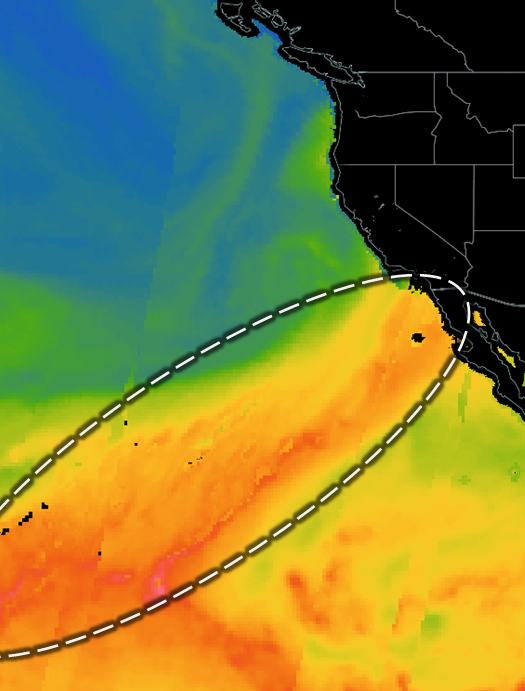
\includegraphics[width=\textwidth]{./ch1/images/ar}\\
    {\scriptsize Credit: NASA}
    \end{minipage}
\end{frame} % Intro

\note{
    EVT is
    \begin{itemize}
    \item Tails - Rather than focusing on the main mass, or \emph{normal behavior}.
    \item Beyond - We have limited data, but are interested in how 'how bad' it could be.
    \end{itemize}
    Applications are myriad.
    \begin{itemize}
        \item Weather
        \begin{itemize}
            \item Atmospheric rivers, such as IVT, which is responsible for the bulk of precipitation in California
            \item Storm surge---things like overtopping dykes, massive flooding events.
        \end{itemize}
        \item Finance
        \begin{itemize}
            \item Mortgage forclosures---unanticipated dependence in foreclosures precipitated securities failures, which precipitated the 2008 banking crisis.
        \end{itemize}
        \item Insurance
        \begin{itemize}
            \item Geographic dependence in risk making insurance prohibitively expensive.
        \end{itemize}
    \end{itemize}
    }

\begin{frame}
    \frametitle{Fisher-Tippet-Gnedenko Thm.}
    For $w_n \stackrel{iid}{\sim} F$:
    \begin{itemize}
    \item If $a_N$, $b_N$ exist such that:
    \[
        \lim\limits_{N\to\infty} \mathbb{P}
            \left[\frac{\vee_{n=1}^N w_n - b_N}{a_N} \leq w\;\right] 
                \;=\; \lim\limits_{N\to\infty}F^N(a_Nw + b_N) 
                \;=\; G(w),
    \]
    Then $G$ is \emph{max-stable}, and $F$ in its \emph{domain of attraction}.
    %\pause
    \item 3 possible forms - \citet{frechet1927,fisher1928,gumbel1942}
    %\pause
    \item One Unifying Form - \emph{GEV} \citet{jenkinson1955}
    \[
        G(w) = \exp\left\lbrace-\left[
            1 + \xi\left(\frac{w - b}{a}\right)
            \right]^{-\frac{1}{\xi}}\right\rbrace
    \]
    \end{itemize}
\end{frame} % Fisher-Tippett-Gnedenko

\note{
    \begin{itemize}
    \item Little history:

    \item In Late 1920's through early 1940's, work by Frechet, Fisher and Tippet, Mises, 
        and Gnedenko shown that
        \begin{itemize}
            \item if there exists a limiting non-degenerate distribution on 
                the maximum observed value in a sample,
            \item  then that distribution is max-stable, and the generating distribution 
                is in its domain of attraction.
        \end{itemize}
    \item That max-stable distribution will take one of 3 possible forms
    \item which can be reframed in a single unifying form: the generalized extreme value distribution.
    \end{itemize}
}

\begin{frame}
    \frametitle{Pickands-Balkema-De Haan Thm.}  
    {\small
    \citet{pickands1975,balkema1974}
    \begin{itemize}
    \item For $W\sim F$
    \[
        \mathbb{P}\left[W > u + y\mid W > u\right] 
            = \frac{1 - F(u + y)}{1 - F(u)},
    \]
        known as the \emph{exceedance function}.
    %\pause
    \item If $F$ in domain of attraction of a GEV, then
    \[
        \lim\limits_{u\to\infty}\mathbb{P}\left(W \geq u + y \mid x \geq y\right)
        = \lim\limits_{u\to\infty}\frac{1 - F(u + y)}{1 - F(u)} = H(y),
    \]
        where $H$ is generalized Pareto
    %\pause
    \item Generalized Pareto Density:
    \[
        H(y) = 1 - \left(1 + \xi\frac{y - b}{a}\right)^{-\frac{1}{\xi}}.
    \]
    %\pause
    \item If $u$ sufficiently large, excesses above $u$ well approximated by Pareto.
    
    Thus, \emph{Peaks-over-Threshold} analysis.
    \end{itemize}
    }
\end{frame} % Pickands-Balkema-de Haan

\note{
    \begin{itemize}
        \item In mid 1970's, Pickands, and Balkema and De Haan showed that if a 
            distribution was in the domain of attraction of the GEV,
        \item  then excesses above a high threshold in that distribution can be 
            well approximated by Generalized Pareto.
        \item This analysis of excesses over a threshold is often termed 
            \emph{peaks-over-threshold}.
    \end{itemize}
}

\begin{frame}
    \frametitle{Multivariate Pareto Distribution}
    \cite{ferreira2014}
    
    Assume $W_d \sim F_d$
    \begin{itemize}
    \item Standardize $\bm{W}$ according to its marginal distribution
    \[
        Z_d = \left(1 + \xi_d\frac{W_d - b_d}{a_d}\right)_+^{\frac{1}{\xi_d}}
    \]
        Note that $Z_d > 1 \implies W_d > b_d$.
    %\pause
    \item If $F_d$ in DoA of the GEV for all $d = 1,\ldots,D$
    \[
    n\;\mathbb{P}\left(
        \frac{Z_1}{n} \geq z_1 \text{ or }\ldots\text{ or }\frac{Z_D}{n} \geq z_d
        \right) \xrightarrow[n\to\infty]{} \mu\left([0,\bm{z}]^c\right)
    \]
    where $\mu$ is the asymptotic distribution of $Z$ in extreme regions.
    %\pause
    \item $\mu$ features the homogeneity property, $\mu(t\cdot) = t^{-1}\mu(\cdot)$.
    \end{itemize}
\end{frame} % Multivariate Pareto Distribution

\note{
    TO DO
}


\begin{frame}
    \frametitle{Spectral (Angular) Measure}
    \begin{itemize}
    \item For $B \in \mathbb{S}_{\infty}^{D-1}$, define the \emph{Spectral Measure}
    \[
        \Psi(B) = \mu\left\lbrace \bm{z} : R(\bm{z}) > 1,\;V(\bm{z}) \in B\right\rbrace
    \]
    where $R(\bm{Z}) = \bigvee_{d = 1}^D Z_d$,  and $V(\bm{Z}) = \bm{Z}\,/\,R(\bm{Z})$
    %\pause
    \item Then
    \[
        \mu\left\lbrace\bm{z} : R(\bm{z}) > r, V(\bm{z}) \in B\right\rbrace = r^{-1}\Psi(B)    
    \]
    Thus $R(\bm{Z})$ is independent of $V(\bm{Z})$.
    %\pause
    \item Thus to complete the probability measure
    \[
        \Phi(B) = \mathbb{P}\left(\bm{V} \in B \mid R > 1\right) = 
            \frac{\Psi(B)}{\Psi\left(\mathbb{S}_{\infty}^{D-1}\right)}
    \]
    \end{itemize}
\end{frame} % Spectral Measure

\note{
    TO DO
}

\section[Multivariate PoT]{BNP Inference for Multivariate PoT Models}
\subsection{Estimation of the Angular Measure}
\begin{frame}
    \frametitle{Separation of Angular and Radial Components}
    {\small
    for $\bm{w}_n$, $n = 1,\ldots,N$
    \begin{enumerate}
        \item Specify $b_d$, estimate $a_d$, $\xi_d$    
            marginally for $d = 1,\ldots,D$
        %\pause
        \item Standardize according to
        \[
            z_{nd} = 
                \left(1 + \xi_d\frac{w_{nd} - b_d}{a_d}\right)_+^{\frac{1}{\xi_d}}        
        \]
        %\pause
        \item Calculate
        \[
            r_n = \bigvee_{d = 1}^D z_{nd},\hspace{1cm}\bm{v}_n = 
                \frac{\bm{z}_n}{r_n}
        \]
        %\pause
        \item Filter $n : r_n \geq 1$
        \[
            r_n \mid r_n \geq 1 \sim \text{Pareto}(1)
        \]
        %\pause
        \item $\bm{Z} \sim \text{MV Pareto}(1)$.  Dependence structure of 
            $\bm{Z}$ expressed in $\bm{V} \in \mathbb{S}_{\infty}^{D-1}$.
    \end{enumerate}
    }
\end{frame} % Separation of R,V

\note{
    \begin{itemize}
    \item I hope you liked that extremely brief review of theory.  Now we get to application.

    \item We set thresholds marginally at a specified quantile, then estimate the scale and extremal index.

    \item We then standardize each observation.  Standardized observations in excess of the threshold are standard Pareto.

    \item Calculate $r$ and $\bm{v}$, and filter data such that $r > 1$.

    \item Since $r$ is independent of $\bm{v}$, and the distribution of $r$ is known, the inference left to us is identifying the dependence structure of $\bm{z}$, which is expressed through $\bm{v}$.

    We need an angular distribution to model $\bm{v}$, on the positive orthant of the unit hypercube.
    \end{itemize}
}

\begin{frame}
    \frametitle{The $\mathcal{L}_p$-Norm Sphere}
    \begin{columns}
        \begin{column}{.49\textwidth}
            {\small 
            \begin{itemize}
                \item $\mathcal{L}_p$-Norm
                \[
                    \lVert \bm{s} \rVert_p = 
                        \left[{\scriptsize \sum}_{d = 1}^D s_d^p\right]^{\frac{1}{p}}
                \]
                %\pause
                \item Positive Orthant of Unit Sphere under $\mathcal{L}_p$-Norm
                \[
                    \mathbb{S}_p^{D-1} = \left\lbrace 
                        \bm{s} : \bm{s} \in \mathbb{R}_+^D, \; \lVert \bm{s}\rVert_p = 1
                        \right\rbrace
                \]
                %\pause 
                \item In the limit
                \[
                    \mathbb{S}_p^{D-1} 
                        \xrightarrow[p\to\infty]{} \mathbb{S}_{\infty}^{D-1}
                \]
            \end{itemize}
            }
        \end{column}%
        \hfill
        \begin{column}{.49\textwidth}
            \begin{center}
                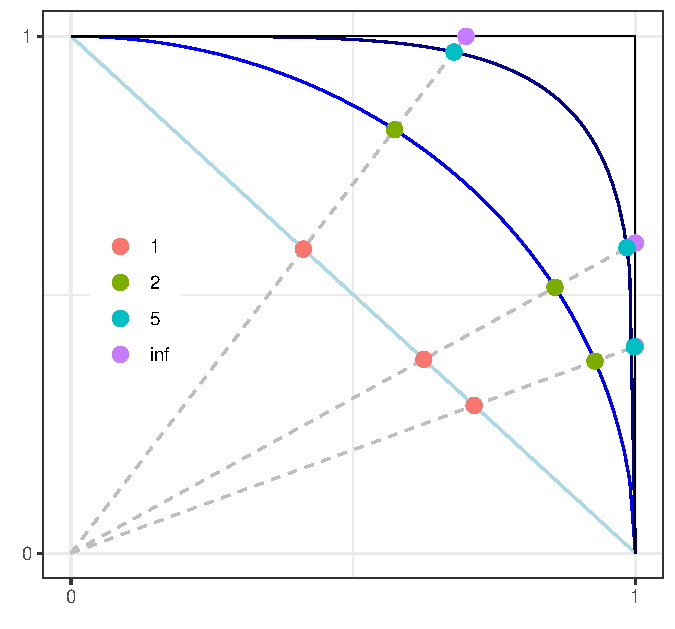
\includegraphics[
                    height = \frametextheight, width = \frametextheight
                    ]{./ch1/images/p_project}
            \end{center}
        \end{column}
    \end{columns}
\end{frame} % L_p-norm sphere

\note{
    \begin{itemize}
        \item So let's build an angular distribution.
        \item Let's consider building a distribution on the positive orthant of the unit $p$-norm Sphere.
        \item As in the limit, the $p$-norm sphere approaches the $\infty$-norm sphere.
    \end{itemize}
}

\begin{frame}
    \frametitle{Projection onto the Unit Sphere}
    {\footnotesize
    \begin{itemize}
        \item We want to take a distribution from 
            $\mathbb{R}_+^D$ to $\mathbb{S}_p^{D-1}$
        %\pause
        \item For finite $p$,
        \[
            Y_D = \left(1 - {\scriptsize \sum}_{d = 1}^D 
                Y_d^p \right)^{\frac{1}{p}}
        \]
        %\pause
        \item Transform to $R$, $\bm{V}$
        \[
            T(X_1,\ldots,X_D) \;=\; 
                \left(\lVert \bm{X}\rVert_p, \frac{X_1}{\lVert \bm{X}\rVert_p},
                    \ldots, \frac{X_{d-1}}{\lVert \bm{X}\rVert_p}\right) 
                \;=\; (R,Y_1,\ldots,Y_{D-1})
        \]
        %\pause
        \item Inverse Transformation:
        \[
            T^{-1}(R,Y_1,\ldots,Y_{D-1}) = 
                \left(RY_1,\ldots,RY_{D-1},
                    R\left(1 - {\scriptsize \sum}_{d = 1}^{D-1}Y-d^p
                        \right)^{\frac{1}{p}}\right) = (X_1,\ldots,X_D)
        \]
        %\pause
        \item Determinant of the Jacobian:
        \[
            \lvert J\rvert = R^{D-1}\left[Y_D + 
                {\scriptsize \sum}_{d = 1}^{D-1}Y_d^pY_D^{1-p}\right]
        \]
    \end{itemize}
    }
    
    \vfill
    \hyperlink{pgpareto:jacobian}{\beamerbutton{Jacobian Details}}
\end{frame} % Projection onto unit Sphere

\note{
    \begin{itemize}
        \item If we want to project a distribution from the positive orthant of the reals, 
            to the positive orthant of the unit sphere, then we need a transformation
            that gets us there.
        \item Consider $\bm{X} = \bm{R}\bm{Y}$ where $R$ is the radius, and $Y$ is the 
            angular portion of $X$ that exists on the unit $p$-norm sphere.
        \item we have $D$ degrees of freedom.  We take one degree of freedom as the radius,
            and one dimension needs to be a function of the others.
        \item If we invert that, take the Jacobian, and find its determinant...
        \item We are left with this.  Note $R^{D-1}$ is just hanging out, and the rest is scalar.
        \item So we need a distribution where $R$ can be integrated out, and can readily
            absorb that $R^{D-1}$ from the Jacobian.
    \end{itemize}
}

\subsubsection{Projected Gamma Distribution}

\begin{frame}
    \frametitle{Projected Gamma}
    \label{pgpareto:projectedgamma}
    \begin{itemize}
    \item Starting from a product of independent gammas,
        \[
        f\left(T(\bm{x})\right) = f(r,\bm{y}) = \prod_{d = 1}^D
            \text{Ga}(ry_d\mid\alpha_d,\beta_d)\times \lvert J \rvert
        \]
    %\pause
    \item Integrate out $r$:
        \[
        f(\bm{y}) = \int_{0}^{\infty}
            \prod_{d = 1}^D\left[\frac{\beta_d^{\alpha_d}}{\Gamma(\alpha_d)}
            (ry_d)^{\alpha_d - 1}
            \exp\left\lbrace-\beta_dry_d\right\rbrace\right] \times 
            r^{D-1}\left[y_d - \sum_{d = 1}^{D-1}y_d^pY_D^{1-p}\right]
            \;\text{d}r
        \]
    %\pause
    \item Left with a distribution on $\bm{y} \in \mathbb{S}_{\infty}^{D-1}$
    \[
    \mathcal{PG}(\bm{y}\mid\bm{\alpha},\bm{\beta}) = 
        \prod_{d = 1}^D\left[\frac{\beta_d^{\alpha_d}}{\Gamma(\alpha_d)}
            y_d^{\alpha_d - 1}\right]
        \times \left[y_d - \sum_{d = 1}^{D-1}y_d^py_D^{1-p}\right]
        \times \frac{\Gamma(\sum_{d = 1}^D\alpha_d)}{
            \left(\sum_{d = 1}^{D}\beta_dy_d\right)^{\sum_{d = 1}^D\alpha_d}}
    \]
    \end{itemize}
    \hyperlink{pgpareto:projgammainference}{\beamerbutton{Recovery of Independence}}
\end{frame} % Projected Gamma Distribution

\note{
    \begin{itemize}
        \item Enter the gamma distribution.
        \item If we start from a product of gammas, even with that Jacobian,
        we can integrate out $R$ in closed form.
        \item And are left with this: a nice closed form density.
        \item This distribution has some rather nice properties
        \begin{itemize}
            \item For one, If we re-introduce the latent $r$, we can marginalize 
                inference on its shape and rate parameters.
        \end{itemize}   
    \end{itemize}
}

\begin{frame}
    \frametitle{Choice of a Norm}
    \begin{itemize}
    \item $\bm{V} \in \mathbb{S}_{\infty}^{D-1}$.
        \[
            \mathbb{S}_p^{D-1} \xrightarrow[p\to\infty]{} 
                \mathbb{S}_{\infty}^{D-1}
        \]
    %\pause
    $T^{-1}(\bm{X})$ not differentiable at $p = \infty$.\vspace{0.25cm}~
    %\pause
    \item Recall the Jacobian:
        \[
        \lvert J\rvert = R^{D-1}\left[Y_D +
            {\scriptsize \sum}_{d = 1}^{D-1}Y_d^pY_D^{1-p}\right]
        \]
    %\pause
    \item Density diverges as $Y_D\to 0$.
    %\pause
        \item So select large but finite $p\;\longrightarrow\;p=10$
    \end{itemize}
\end{frame}

\note{
    \begin{itemize}
        \item Unfortunately it's not all gumdrops and rainbows.
        \item The phenomena we want to study lives on $\mathbb{S}_{\infty}^{D-1}$
        \item But the transformation is not differentiable.
        \item Further, note $Y_D^{1-p}$ in the determinant of the Jacobian.
        \item for small $Y_D$, that goes to infinity---the density diverges.
        \item So we select a finite but reasonably large $p$.
    \end{itemize}
}

\begin{frame}
    \frametitle{Angular Data Model}
    \label{pgpareto:angulardatamodel}
    {\small
    \begin{itemize}
    \item Basic Model \emph{(DPPG)}
        \[
            \bm{y}_n\mid\bm{\alpha} \sim 
            \mathcal{PG}\left(\bm{y}\mid\bm{\alpha}_n,\bm{\beta}_n\right)
            \hspace{1cm}
            \bm{\alpha}_n \sim 
            \mathcal{DP}(\bm{\alpha}\mid\eta, G_0)
        \]
    %\pause
        For identifiability, $\beta_{\jmath 1} := 1$\hspace{1cm}
            \emph{DPPRG}: $\beta_{\jmath d} = \beta = 1$ for all $d$\\~
    %\pause
    \item Choice of Centering Distribution
        \begin{description}
            \item[\emph{DPPG-G}] Product of Gammas
                \[
                G_0 = \prod_{d = 1}^D\text{Ga}\left(\alpha_d\mid \xi_d,\tau_d\right)
                \times\prod_{d=2}^D\text{Ga}\left(\beta_d\mid \zeta_d,\sigma_d\right)
                \]
                With gamma priors on $\xi,\tau,\zeta,\sigma$\\~
            \item[\emph{DPPG-LN}] Log-Normal
                \[
                G_0 = \mathcal{LN}\left(\bm{\alpha}\mid\mu,\Sigma\right) \times \prod_{d = 2}^D\text{Ga}\left(\beta_d\mid \zeta_d,\sigma_d\right)
                \]
                With Normal prior on $\mu$, Inverse Wishart prior on $\Sigma$.
        \end{description}
    \end{itemize}
    }
    \hyperlink{pgpareto:pginference}{\beamerbutton{Full Conditionals for DPPG-G}}
\end{frame} % Angular Data Model

\note{
    \begin{itemize}
        \item Now we get to specifying an angular data model.
        \item We're using a Bayesian non-parametric prior here; in this case a Dirichlet process,
            with projected gamma as a kernel distribution.
        \item We're also considering the idea of a projected \emph{restricted} gamma, with the
            rate parameters set to 1.
        \item And choices of product-of-gammas and log-normal as centering distribution
            with appropriate priors.
    \end{itemize}
}

\subsection{Model Comparison}

\begin{frame}
    \frametitle{Comparing Model Fidelity on $\mathbb{S}_{\infty}^{D-1}$}
    Energy Score~-~\cite{gneiting2007}
    \label{pgpareto:energyscore}
    \begin{minipage}{0.7\textwidth}
    {\footnotesize 
    \begin{itemize}
    \item Generalization of \emph{Continuous Ranked Probability Score} 
        to multiple dimensions
        \[
        \text{ES}\left(P,\bm{x}_n\right) =  
            \mathbb{E}_p g\left(\bm{X}_n, \bm{x}_n\right)
            - \frac{1}{2}\mathbb{E}_p g\left(\bm{X}_n,\bm{X}_n^{\prime}\right)
        \]
        where $g$ is a negative definite kernel.\footnote{A negative 
        definite kernel satisfies symmetry in its arguments, and 
        $\sum_{i = 1}^N\sum_{j = 1}^N \alpha_i\alpha_j g(\bm{x}_1,\bm{x}_2) \leq 0$ 
        for all $x_1,x_2$, for all $\alpha_i$ such that $\sum_{i = 1}^N\alpha_i = 0$.
        }
    %\pause
    \item With appropriate (negative definite) kernel 
        $\Longrightarrow$ \emph{proper} scoring rule
    %\pause
    \item Need an appropriate kernel in $\mathbb{S}_{\infty}^{D-1}$.  Geodesic distance?
    %\pause
    \item Not geodesic distance.  Too costly.
    %\pause
    \item Upper bound on geodesic distance - Euclidean norm on 1d Rotation
    \end{itemize}
    \vfill
    }
    \end{minipage}%
    ~\hfill
    \begin{minipage}{0.29\textwidth}
    \begin{center}
        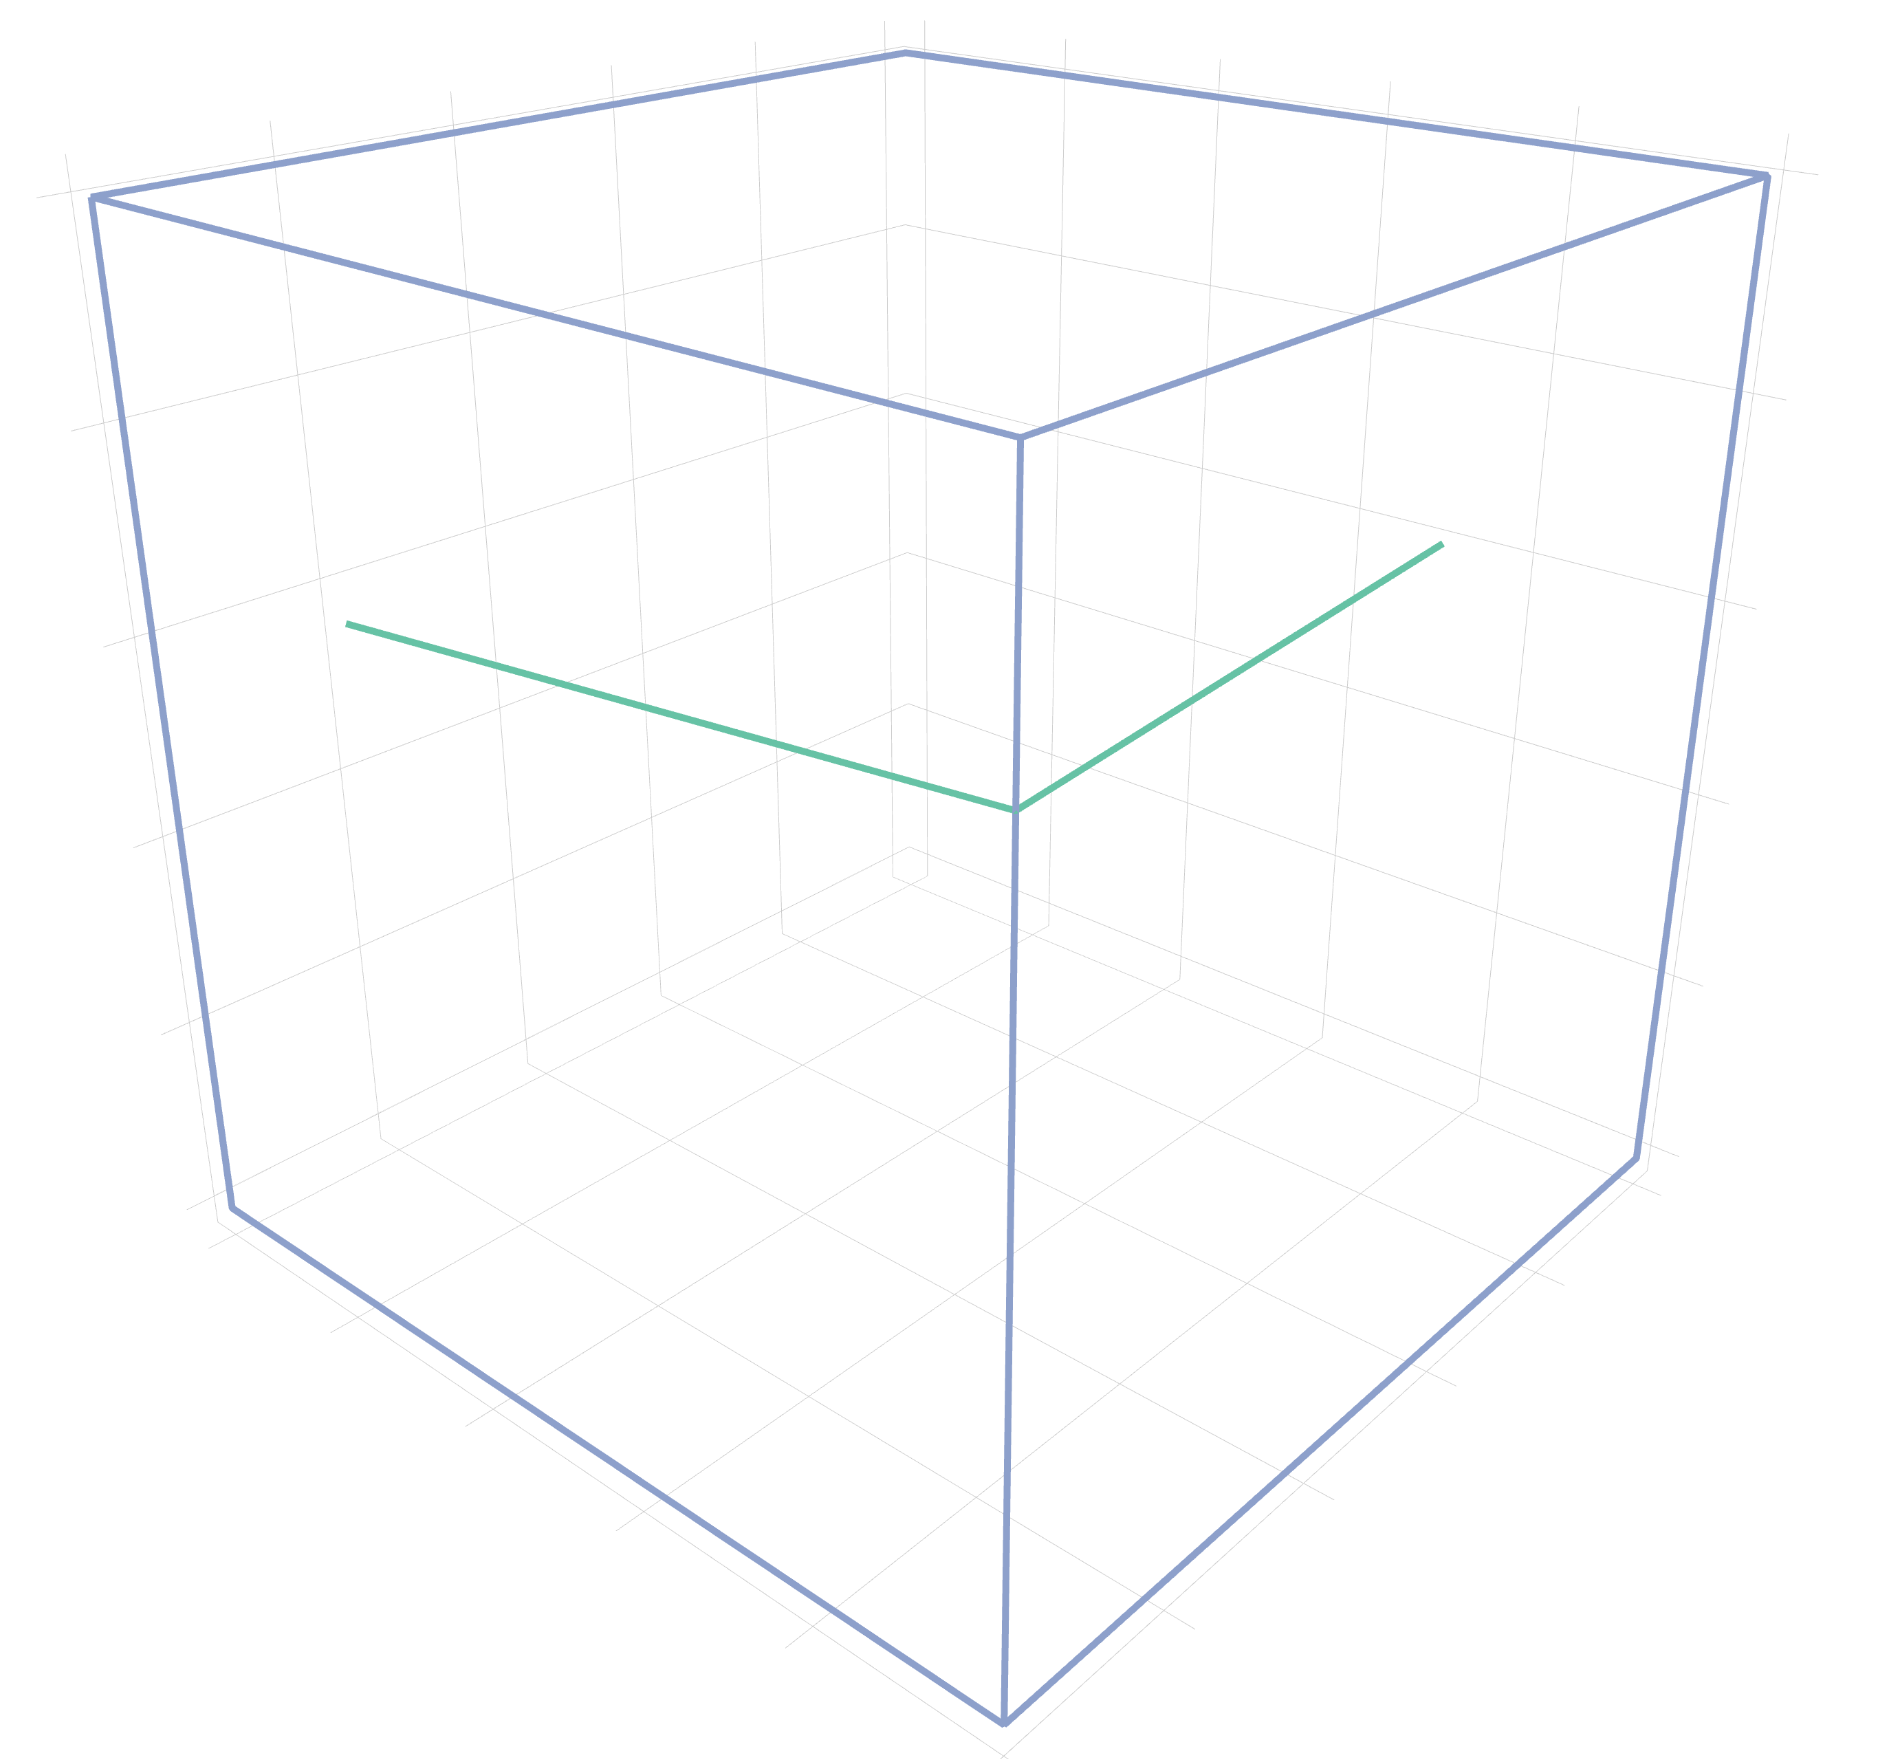
\includegraphics[width=\textwidth]{ch1/images/1drot}
    \end{center}
    \hyperlink{pgpareto:notgeodesic}{\beamerbutton{Not Geodesic}}
    \hyperlink{pgpareto:kerneldetails}{\beamerbutton{Kernel Details}}
    
    \end{minipage}
\end{frame} % Model Comparison

\note{
    \begin{itemize}
        \item We have multiple candidate models.  We need a means of testing 
            model fidelity.  We consider energy score.
        \item Energy score is based on pairwise distances---or some analogue to distance, at least.
        \item We desire a distance metric appropriate to $\mathbb{S}_{\infty}^{D-1}$.  Geodesic distance?
        \item Not as it turns out.  Too costly.
        \item An upper bound on geodesic distance is computationally feasible.  All faces of the
            unit hypercube are pairwise adjacent, we can just calculate the distance from the source to 
            the optimal vertex, and then from the vertex to the target.
        \item or just rotate the target face into the same plane as the source face, and a straight line
            passes through the optimal vertex.  Which means we just use Euclidean distance between the 
            source and rotated target.
    \end{itemize}
}

\subsubsection{Model Recovery}

\begin{frame}
    \label{pgpareto:simstudy}
  \frametitle{Simulation Study - Energy Score}
  \begin{center}
    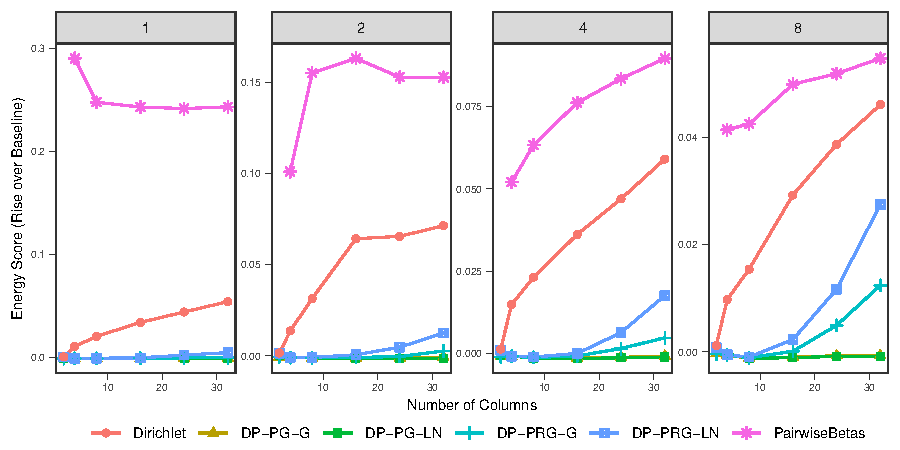
\includegraphics[height=0.9\frametextheight]{./ch1/images/sim_es_rise}
  \end{center}
  \hyperlink{pgpareto:simstudydetails}{\beamerbutton{Details}}
\end{frame} % Simulation Study - Energy Score

\note{
    \begin{itemize}
        \item TODO
    \end{itemize}
}

\subsection{Integrated Vapor Transport}

\begin{frame}
  \frametitle{Integrated Vapor Transport (IVT)}
  \begin{minipage}{.7\textwidth}
    \begin{itemize}
        \item Atmospheric rivers~\citep{ralph2013,ralph2018}
            \begin{itemize}
                \item Concentrated water vapor in atmosphere
                \item Huge amounts of water
                \item Predominant source of precipitation for 
                    inland California
                \item Extreme behavior has large implications 
                    for land use, agriculture, flood prevention / mitigation
            \end{itemize}
        \item The data~\citep{guan2015}
            \begin{itemize}
                \item 42 years of daily average of total water content 
                    in atmospheric column above grid cell
                \item Grid cells cover coast of California in two 
                    spatial resolutions
                    \begin{description}
                        \item[ERA-Interim] 8 Cells
                        \item[ERA5] 47 Cells
                    \end{description}
                \item subset to rainy season (November to March)
                \item Decorrellated by dropping all but max in a sequence of threshold exceedences
            \end{itemize}
    \end{itemize}
  \end{minipage}
  ~\hfill
  \begin{minipage}{.25\textwidth}
    \centering
    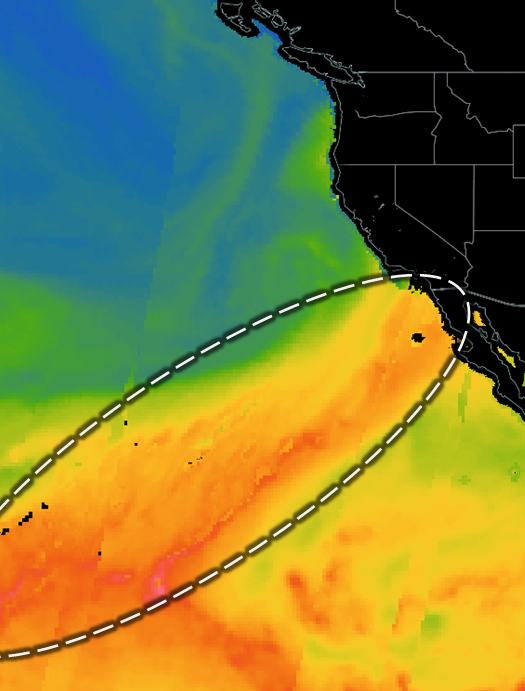
\includegraphics[width=\textwidth]{./ch1/images/ar}\\
    {\scriptsize Credit: NASA}
   \end{minipage}
\end{frame} % IVT Intro

\note{
    \begin{itemize}
        \item Now to the motivating example of the first paper.
        \item We looked at the integrated vapor transport, which is an atmospheric 
            river that carries moisture inland over California.  It's responsible
            for the lion's share of precipitation in the western US.
        \item An observation is one day's average total water content in atmospheric
            columns above each grid cell.
        \item We have 42 years of such data, in two resolutions, 8 and 47.
        \item We've subset the data to specifically the rainy season, and decorrelated it.
    \end{itemize}
}

\begin{frame}
    \frametitle{IVT Grid}
    \begin{figure}[h]
        \begin{minipage}{.49\textwidth}
            \centering
            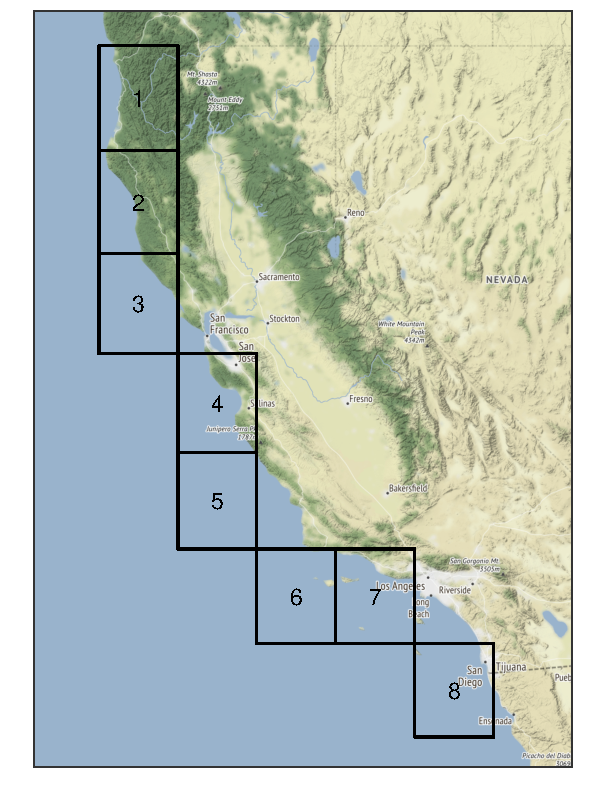
\includegraphics[height=\frametextheight]{./ch1/images/erai_grid}
        \end{minipage}
        \begin{minipage}{.49\textwidth}
            \centering
            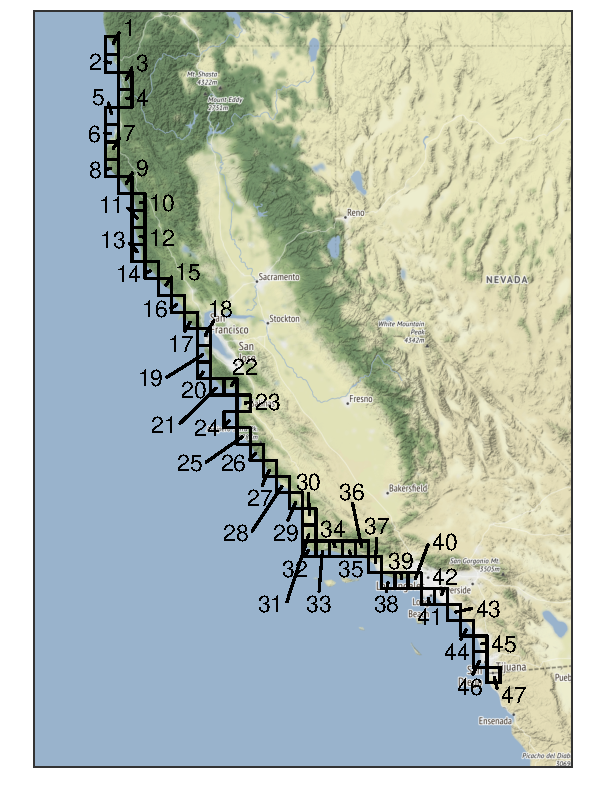
\includegraphics[height=\frametextheight]{./ch1/images/era5_grid}
      \end{minipage}
      \caption{(Left) ERA-Interim Spatial Grid; (Right) ERA5 Spatial Grid.}
  \end{figure}
\end{frame} % IVT Grid Map

\note{
    \begin{itemize}
        \item Here we see that spatial grid.  
        
        \item Lower resolution means a \emph{bigger} area for each grid cell.  
        
        \item Bigger area means deviations in average water content are going to 
            be less pronounced, since they're averaging over a larger area.
    \end{itemize}
}

\subsubsection{IVT - Extremal Dependence}

\begin{frame}
  \frametitle{Pairwise Extremal Dependence Coefficients}
    \begin{itemize}
      \item A summary measure of extremal dependence
      \begin{equation*}
        \chi_{kl} = \lim\limits_{u\to\infty}\mathbb{P}\left(Z_k > u\mid Z_l > u\right).
      \end{equation*}
      %\pause
      \item Bounded to $[0,1]$
        \begin{itemize}
          \item $0$ represents asymptotic independence
          \item A Pareto model can not represent asymptotic independence
        \end{itemize}
      %\pause
      \item Reformulated to unit hypercube
        \begin{equation*}
          \chi_{k\ell} = \mathbb{E}\left[\frac{V_k}{\mathbb{E}(V_k)}{\bigwedge}\frac{V_{\ell}}{\mathbb{E}(V_{\ell})}\right]
        \end{equation*}
        Where $\bm{V} = \bm{Z}\,/\, \lVert\bm{Z}\rVert_{\infty}$
    \end{itemize}
\end{frame} % Pairwise Extremal Dependence coefficients - Intro

\note{
    \begin{itemize}
        \item One of the things we can do with our fitted model is assess pairwise dependence.
        \item In fact, we can do much cooler things, but in the interest of time, I'll leave 
            presenting those to paper 3.
        \item Think of pairwise dependence coefficients as somewhat loosely related to correlation.
        \item It's a number, that tells how closely related extremes in one dimension are with another.
        \item 0 means asymptotic independence, but a Pareto model (which is what we have) can never represent
            asymptotic independence.
    \end{itemize}
}

\begin{frame}
  \frametitle{IVT - Extremal Dependence}
  \centering
  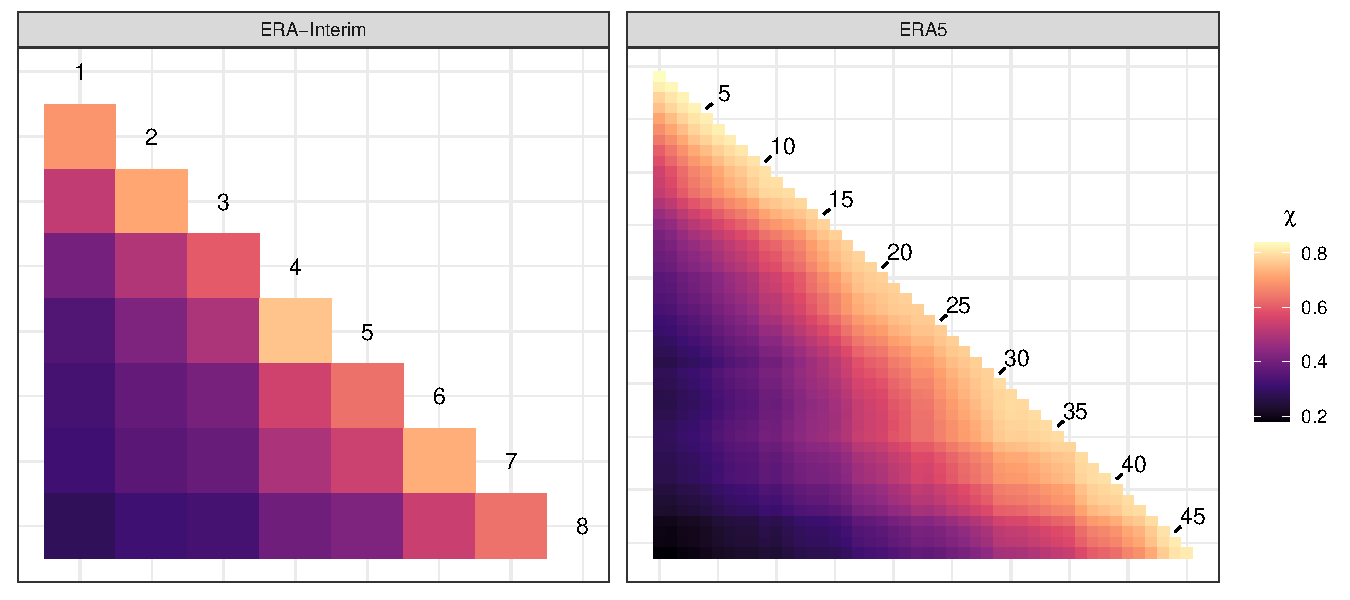
\includegraphics[width=0.99\linewidth]{./ch1/images/chi_ij_c}
\end{frame} % Pairwise Extremal Dependence coefficients - Plot

\note{
    \begin{itemize}
        \item This is pairwise extremal dependence plot for both resolutions.  We have some \emph{clusters} 
            of relatively high dependence.
        \item This model makes no assumptions with regard to geography.  But here we observe strong but
            heterogeneous geographic dependence.
    \end{itemize}
}

% \subsection{Conclusion}

\section[Anomaly Detection]{Anomaly Detection in PoT Settings and Angular Representations of Categorical Data}
\subsection{Introduction}

\begin{frame}
    \frametitle{What is an anomaly?}
    \label{ndpg:anomaly}
    {\small
    \begin{itemize}
        \item Anomalies are:
        \begin{itemize}
            \item Observations with large outliers?
            \item Observations with outsized effects?
            \item Data that is \emph{different}.
            \item Data from regions of data sparsity.
            \item Anomalies may tend to exist at the edge of \emph{extreme} regions.
        \end{itemize}
        \item Desire anomaly \emph{scores}--larger$\rightarrow$more anomalous
        \item A General Anomaly Score:
        \[
            \mathcal{S}_n = \left[\int_{\Theta}f(x_n\mid\theta)\,dG(\theta\mid\bm{x})\right]^{-1}
        \]
        %\pause
        \item An Extremal Anomaly Score:
        \[
            \mathcal{S}_n = \mathcal{S}_{n,r} \times \mathcal{S}_{n,\bm{v}}
                = f_r(r_n)^{-1}\times \left[\int_{\Omega}f_{\bm{v}}(\bm{v}_n\mid\bm{\alpha})\,\text{d}G(\bm{\alpha}\mid\bm{v})\right]^{-1}
        \]
        where $r_n\sim\text{Pareto}(1)\;\longrightarrow\;f_r(r_n) = r_n^{-2}$.
    \end{itemize}
    }
    \hyperlink{ndpg:anomalymethods}{\beamerbutton{Methods Expansion}}
\end{frame} % What is an anomaly?

\note{
    \begin{itemize}
        \item One of the applications we were interested in using extreme analysis was 
            anomaly detection.
        \item Now, in regards to extreme analyis, a good question to ask is what is an 
            anomaly?
        \item In a regression context, this might be observations with large outliers?  
            Or have large effects on inference?
        \item For our purpose, we consider anomalous data to have a different generating
            distribution than \emph{normal} data.
        \item We expect it to appear in regions of data sparsity---potentially in extreme
            regions to a greater extent.
        \item We desire an interpretable anomaly score--larger means more anomalous.
        \item this is relatively easy to accomplish as the reciprocal of the density.
        \item In an extreme case, given the separation of radial and angular components,
            we can seprate the radial and angular scores.  The radial score is easy.
    \end{itemize}
}

\subsection{Novelty Detection Methods}

\begin{frame}
    \frametitle{Estimation of the Angular Score}
    \label{ndpg:estimationofangularscore}
    \begin{itemize}
        \item Similar angular data model as previous
        \begin{itemize}
            \item Pitman-Yor process for greater control over clustering
            \item $G_0 = \mathcal{LN}\left(\bm{\alpha}\mid\mu,\Sigma\right)$ 
                for consistency later
        \end{itemize}
        \item Need an angular density
        \item Density on $\mathbb{S}_{\infty}^{D-1}$ not available
        \item Density on $\mathbb{S}_p^{D-1}$ problematic: no unique transformation
        \item Gamma density is problematic: For $\alpha < 1$,
        \[
        \text{Ga}(x\mid\alpha, 1) \xrightarrow{x\to 0}{}\infty
        \]
        \item Multivariate extreme data tends to exist near edges, with some $v_d = 0$
        \item Alternate density estimator?
    \end{itemize}
    \hyperlink{ndpg:angulardatamodel}{\beamerbutton{Angular Data Model Details}}
\end{frame}

\note{
    \begin{itemize}
        \item Now, we want to create an angular score.
        \item Ideally, this would be the reciprocal of the posterior predictive density 
            as stated.
        \item So we use a similar BNP mixtures of projected restricted gamma model as previous, 
            with a Pitman-Yor process prior for greater control over the clustering.
        \item For consistency later, we'll use a log-normal centering distribution for the shapes.
        \item Now the problems:
        \begin{itemize}
            \item Density on the unit hypercube isn't available.
            \item Density on the unit $p$-norm sphere is problematic, for two reasons:
                The transformation isn't unique, and the edge-seeking behavior of the gamma 
                when the shape is less than 1.
            \item multivariate data tends to exist near edges.
        \end{itemize}
        \item So we need some alternate density estimator?        
    \end{itemize}
}

\begin{frame}
    \frametitle{$k$-Nearest Neighbors}
    \begin{itemize}
        \item Radius to $k$-th nearest neighbor
        \[
            R_k(\bm{v}_n) = g\left(\bm{v}_n,\bm{v}_{N_k(n)}^*\right)
        \]
        where $\bm{v}_{N_k(n)}^*$ is the $k$th nearest neighbor of $\bm{v}_n$ on the posterior predictive sample.
        %\pause
        \item Assume a uniform density within a sphere of radius of $R_k(\bm{v}_n)$
        %\pause
        \item Score:
        \[
            \mathcal{S}_{n,\bm{v}}^{\text{$k$NN}} 
                = \frac{N\pi^{\frac{D-1}{2}}R_k(\bm{v}_n)^{D-1}}{k\Gamma(\frac{D-1}{2} - 1)}
        \]
        the reciprocal of that density.
    \end{itemize}
\end{frame} % KNN

\note{
    \begin{itemize}
        \item  Well, there's many options, but two readily available are $k$-nearest neighbors 
            and kernel density estimation.
        \item $k$-NN assumes a uniform density within a sphere of radius the "distance" to the 
            $k$th nearest neighbor on the posterior predictive sample.
        \item The \emph{distance} we're using is the previously mentioned distance analogue on 
            $\mathbb{S}_{\infty}^{D-1}$
        \item And then the score is the reciprocal of that estimated density.
    \end{itemize}
}

\begin{frame}
    \frametitle{Kernel Density Estimation}
    {\footnotesize
    \begin{enumerate}
        \item General KDE for scalar bandwidth parameter $h$
        \[
        f_n(\bm{x}) = \int_{\Omega}\frac{1}{h}\mathcal{Q}\left(\frac{\bm{x} 
                - \bm{t}}{h}\right)dF_n(\bm{t})
            \approx \frac{1}{Kh}\sum_{k = 1}^K\mathcal{Q}\left(\frac{\bm{x} 
                - \bm{x}_k^*}{h}\right)
        \]
        where $\bm{x}_k^*$ are replicates from $F$.  We use normal distribution 
            for $\mathcal{Q}$
        %\pause
        \item Silverman's Rule of Thumb
        \[
            \hat{h} = \left(\frac{4}{D + 2}\right)^{
                \frac{1}{D + 4}}K^{-\frac{1}{D+4}}
                \hat{\sigma}
        \]
        where $\hat{\sigma}$ refers to empirical standard deviation.
        %\pause
        \item Recall for R.V. $X$, 
            $\mathbb{E}\left[\lVert X_{\jmath} - X_k\rVert_2\right] = 2\text{Var}(X)$.  
            Then
        \[
            \hat{\sigma} = 
                \sqrt{\frac{1}{2K(K-1)}\sum_{\jmath \neq k}
                    g\left(\bm{v}_{\jmath}^*,\bm{v}_k^*\right)}
        \]
        %\pause
        \item Score:
        \[
        \mathcal{S}_{n,\bm{v}}^{\text{kde}} \propto 
            \left[\sum_{k=1}^K\exp\left\lbrace-\left(
                \frac{g(\bm{v}_n,\bm{v}_k^*)}{h}\right)^2\right\rbrace\right]^{-1}
        \]
    \end{enumerate}
    }
\end{frame} % Kernel Density Estimation

\note{
    \begin{itemize}
        \item KDE is a little more interesting.
        \item $Q$ is a kernel function.  The estimation is based on pairwise distances
            (again using the term distance loosely).
        \item Silverman's rule of thumb is about estimation of the bandwidth parameter.
            It requires an estimate of standard deviation.
        \item This is a multivariate distribution.  Standard deviation isn't defined.
            But we do have those pairwise distances, which are univariate.
        \item So being wildly disrespectful to theory, we come up with this estimator of
            standard deviation.
        \item And the score is then going to the reciprocal of the estimated KDE.
    \end{itemize}
}

\subsection{Binary and Categorical Data}

\subsubsection{Angular Representations of Categorical Data}

\begin{frame}
    \frametitle{Categorical Distributions}
    \label{ndpg:categoricaldistributions}
    {\small 
    \begin{itemize}
        \item Dirichlet-Multinomial Distribution
            \[
            \mathcal{DM}(\bm{c}\mid\bm{\alpha}) = 
                \int_{\bm{\pi}}\mathcal{M}(\bm{c}\mid\bm{\pi})\,
                \mathcal{D}(\bm{\pi}\mid\bm{\alpha})\,\text{d}\bm{\pi}
            \]
        %\pause
        \item Dirichlet-Categorical Distribution
            \[
            \bm{c}\mid\bm{\alpha} \sim 
            \mathcal{DC}(\bm{c}\mid\bm{\alpha}) = 
            \frac{
                \Gamma(\sum_{d=1}^D \alpha_{d})
                }{
                \Gamma(1 + \sum_{d = 1}^D\alpha_{d})
                }
            \prod_{d = 1}^D 
            \frac{\Gamma(c_{d} + \alpha_{d})}{\Gamma(\alpha_{d})}
            \]
        \item Let $\bm{c}_m$ be categorical RV with $D_m$ categories in one-hot:
        \[
        \mathcal{CDC}(\bm{c}\mid\bm{\alpha}) = 
        \prod_{m = 1}^M \mathcal{DC}(\bm{c}_m\mid\bm{\alpha}_m)
        \]
        \item The Model:
        \[
        \bm{c}_n \sim \mathcal{CDC}\left(\bm{c}\mid\bm{\alpha}_n\right) \hspace{1cm}\bm{\alpha}_n \sim G \hspace{1cm} G \sim \mathcal{PY}\left(\omega,\eta,G_0\right)
        \]
        where $G_0 = \mathcal{LN}_D\left(\bm{\alpha}\mid\mu,\Sigma\right)$.
    \end{itemize}
    }
    \hyperlink{ndpg:categoricaldatamodel}{\beamerbutton{Categorical Data Model Details}}
\end{frame} % Categorical Distributions

\note{
    \begin{itemize}
        \item Sadly canonical "anomaly detection" datasets appropriate to this model don't seem to exist.
        \item Financial datasets, such as wire fraud, where I believe this method would shine
            are not available.
        \item So we considered how to expand the applicability of the method to other data.
        \item And we considered the idea of an angular representation of categorical data.
        \item The Dirichlet multinomial distribution is what's left when you integrate out
            a dirichlet RV from a multinomial with a Dirichlet prior.
        \item As a categorical RV is a multinomial with $N = 1$, we can simplify that to this form.
        \item Then our categorical data model is a BNP mixture of concatenated Dirichlet-Categorical
            RV's, with a Pitman-Yor prior.  We introduce negative dependence between the categories
            in the prior for $\Sigma$.
    \end{itemize}
}

\subsubsection{Novelty Detection for Categorical Data}

\begin{frame}
    \frametitle{Novelty Scores}
    \label{ndpg:noveltyscores}
    % \begin{itemize}
    % \item Latent Cluster ID's / Parameters
    Latent Cluster ID's / Parameters
        \[
        \mathbb{P}[\gamma_n = \jmath\mid \bm{\alpha}, \bm{\pi}, \bm{c}_n] = 
        \frac{
            \pi_{\jmath}\,\mathcal{CDC}\left(\bm{c}_n\mid\bm{\alpha}_{\jmath}\right)
            }{
            \sum_{k = 1}^J\,\pi_k\,\mathcal{CDC}\left(\bm{c}_n\mid\bm{\alpha}_k\right)
            }
            \;\;\;\text{ for }\jmath = 1, \ldots, J,
        \]
    where $\bm{\pi}$ is cluster weight.
    
    % \item \emph{Angular} representation of categorical:
    \emph{Angular} representation of categorical data:
        \begin{enumerate}
            \item Take samples of $\gamma_n\mid \bm{\alpha}_k,\bm{\pi}_k,\bm{c}_n$ for $k = 1,\ldots,K$, for $n = 1,\ldots, N$.
            \item Sample $\bm{\varphi}_{nk}\sim \prod_{d = 1}^D\text{Ga}(\varphi_d\mid\alpha_{nkd},1)$
            \item Angular representation is conditional posterior of $\bm{\nu}_n = \bm{T}_{\infty}(\bm{\varphi}_n)$
            \item Simplex representation is conditional posterior of $\bm{\pi}_n = \prod_{m = 1}^MT_1(\bm{\varphi}_{nm})$
        \end{enumerate}
    % \item Scores based on pairwise distances between samples of $\bm{\nu}_n$ and $\bm{\nu}^*$
    Scores based on pairwise distances between samples of $\bm{\nu}_n$ and $\bm{\nu}^*$ (or $\bm{\pi}_n$ and $\bm{\pi}^*$)
    % \end{itemize}\\
    \hyperlink{ndpg:noveltyscoresdetail}{\beamerbutton{Novelty Score Details}}
\end{frame} % Categorical Anomaly Scores setup

\note{
    \begin{itemize}
        \item So what do we mean by an \emph{angular} representation of categorical data?
        \item Well, we can find the latent conditional posterior distribution of the dirichlet-categorical
            shape parameters.
        \item Sampling the conditional posterior predictive, we can then project that onto a unit sphere.
            This representation is what we mean by \emph{angular}.
        \item Then scores are based on pairwise distances between samples from the conditional posterior 
            predictive for a given observation, and the posterior predictive distribution.
        \item Given that we're dealing with a latent distribution here, we can either take its expectation
            sequentially (\emph{hkde}, \emph{hknn}), or simultaneously (\emph{lhkde}, \emph{lskde}).
    \end{itemize}
}

\begin{frame}
    \frametitle{AuROC - Categorical}
    \begin{table}
        \centering
        % latex table generated in R 4.2.2 by xtable 1.8-4 package
% Mon Jan 30 15:17:28 2023
\begin{tabular}{l|rrr|rrrr}
  \toprule
dataset & iso & lof & svm & hknn & hkde & lhkde & lskde \\ 
  \midrule
cover & 0.384 & 0.515 & 0.424 & $\bm{0.586}$ & 0.523 & 0.558 & 0.450 \\ 
  pima & 0.620 & 0.570 & 0.614 & 0.457 & 0.579 & 0.659 & $\bm{0.694}$ \\ 
  solarflare & $\bm{0.893}$ & 0.402 & 0.887 & 0.435 & 0.632 & 0.768 & 0.875 \\ 
  yeast & 0.620 & 0.580 & 0.622 & 0.406 & $\bm{0.708}$ & 0.650 & 0.702 \\ 
   \bottomrule
\end{tabular}

    \end{table}
\end{frame} % Categorical Anomaly Score Performance Data

\note{
    \begin{itemize}
        \item TODO
    \end{itemize}
}

\subsection{Mixed Data}

\begin{frame}
    \frametitle{Mixed Data Model}
    {\small 
    \begin{itemize}
        \item Joint Model:
        \[
        (\bm{y},\bm{c}) \sim \int_{\bm{\alpha}}
            \mathcal{PG}_p(\bm{y}\mid\bm{\alpha}_y,\bm{1})\,
            \mathcal{CDM}(\bm{c}\mid\bm{\alpha}_c)\;\text{d}G(\bm{\alpha})
        \]
        %\pause
        \item Joint Projection:
        \[
            R_n \mid \bm{\alpha} \sim \text{Ga}\left(R\mid\sum_{d = 1}^{D_y} \alpha_{yd}, 1\right)
        \]
        Then $\bm{\nu}_n = T_{\infty}(R_n\bm{y}_n,\bm{\varphi}_{nc})$
        %\pause
        \item \emph{h$k$nn}, \emph{hkde}, \emph{lhkde} as previous.
        %\pause
        \item \emph{lmkde}:
        \[
        \begin{aligned}
            \mathcal{S}_{n,\bm{v}}^{lmkde} &= \mathbb{E}_{\bm{v}^*,\bm{\pi}^*,\bm{\pi}_n}\left[
        \exp
        \left\lbrace 
        -\frac{1}{2}
        \left(
        \frac{g\left(\bm{v}_n, \bm{v}^*\right)}{\hat{h}_{\bm{v}^*}}
        \right)^2
        -\frac{1}{2}
        \left(
        \frac{\lVert\bm{\pi}_n - \bm{\pi}^*\rVert_1}{\hat{h}_{\bm{\pi}^*}}
        \right)^2
        \right\rbrace
        \right]^{-1}\\
        &\approx \left[\frac{1}{K_{\bm{\pi}^*}K_{\bm{\pi}_n}}
            \sum_{\jmath = 1}^{K_{\bm{\pi}_n}}\sum_{k=1}^{K_{\bm{\pi}^*}}
            \exp\left\lbrace-\frac{1}{2}
            \left(\frac{g(\bm{v}_n,\bm{v}_k^*)}{\hat{h}_{\bm{v}^*}}\right)^2
            -\frac{1}{2}\left(
            \frac{\lVert\bm{\pi}_{n\jmath} - \bm{\pi}_k^*\rVert_1}{\hat{h}_{\bm{\pi}^*}}
            \right)^2
            \right\rbrace\right]^{-1}
        \end{aligned}
        \]
    \end{itemize}
    }
\end{frame} % Mixed Data Model

\note{
    \begin{itemize}
        \item To the point: we consider a mixed data model, encompassing both regimes: 
            real and angular data.
        \item We consider a joint projection: categorical and angular data in the same
            space.  To do that, we sample the latent radius from the angular component
        \item then project both together into the same space.
        \item The scores are decided as previous.
        \item We also consider a mixed score.  This score does not consider the
            dependence between the two regimes, so we can consider this as somewhat
            a reality check on the efficacy of the joint projection.
    \end{itemize}
}

\begin{frame}
    \frametitle{AuROC - Peaks-over-Threshold - Mixed Data}
    \begin{table}
        \centering
        % latex table generated in R 4.2.2 by xtable 1.8-4 package
% Mon Jan 30 15:17:28 2023
\begin{tabular}{l|rrr|rrrr}
  \toprule
dataset & iso & lof & svm & hknn & hkde & lhkde & lmkde \\ 
  \midrule
annthyroid & 0.458 & 0.512 & 0.640 & 0.691 & 0.692 & $\bm{0.698}$ & 0.689 \\ 
  cardio & $\bm{0.849}$ & 0.610 & 0.836 & 0.590 & 0.812 & 0.804 & 0.823 \\ 
  cover & 0.606 & 0.512 & 0.684 & $\bm{0.832}$ & 0.698 & 0.719 & 0.714 \\ 
  mammography & 0.594 & 0.616 & 0.725 & 0.675 & $0.750$ & $\bm{0.757}$ & 0.725 \\ 
  pima & 0.530 & $\bm{0.565}$ & 0.511 & 0.525 & 0.525 & 0.524 & 0.522 \\ 
  yeast & 0.427 & 0.579 & 0.560 & $\bm{0.639}$ & 0.522 & 0.540 & 0.542 \\ 
   \bottomrule
\end{tabular}

    \end{table}
\end{frame} % AuROC - Mixed Real

\note{
    \begin{itemize}
        \item So first thing we can identify:  The mixed score is never best, but it's 
            also never terrible.
        \item Our methods for anomaly detection look for observations that are in areas
            of low density.  That means observations unlike other observations.  So they
            won't work well on datasets where the definition of an anomaly doesn't match
            our conceptions.
        \item On the other hand, \emph{hknn} and \emph{hkde} trade blows, but \emph{lhkde}
            is generally superior to \emph{hkde}.  Perhaps the additional information
            offered by the latent conditional posterior, rather than just its expectation, 
            helped.
    \end{itemize}
}

\subsubsection{Rank Transformation}

\begin{frame}
    \frametitle{Relaxing the Assumption of Independence}
    \begin{itemize}
        \item Rank Transformation / Standardization
        \[
            z_{nd} = \frac{1}{1 - \hat{F}(w_{nd})}\
            \hspace{1cm}r_n = \lVert \bm{z}_n\rVert_{\infty}
            \hspace{1cm}\bm{v_{n}} = \frac{\bm{z}_n}{r_n}
        \]
        \item Model
        \[
        (\bm{y}_n,\bm{c}_n,r_n) \sim \int_{\bm{\alpha}}
            \mathcal{PG}_p(\bm{y}_n\mid\bm{\alpha}_{\bm{y}}, \bm{1})\;
            \mathcal{CDM}(\bm{c}_n\mid\bm{\alpha}_{\bm{c}})\;
            \mathcal{P}(r_n\mid\alpha_r)\;
            \text{d}G(\bm{\alpha})
        \]
        \item Scores developed as previously described        
    \end{itemize}
\end{frame} % Rank Data Model

\note{
    \begin{itemize}
        \item  Up to now, we relied on thresholding of the real data, which is required
            in order to separate inference of the radial component from the angular component.
        \item This eliminates from consideration all data that did not exceed the threshold.
        \item If we consider an alternate transformation to standard Pareto, that
            based on rank transform, then we no longer lose that data from consideration
        \item But that does mean we need to include the extremal index as one of the parameters.
            We include it, with the log-normal centering distribution as previously mentioned.
        \item The previously developed scores still work.
    \end{itemize}
}

\begin{frame}
    \frametitle{AuROC - Rank-Transformed - Mixed Data}
    \begin{table}
        \centering
        % latex table generated in R 4.2.2 by xtable 1.8-4 package
% Mon Jan 30 15:17:28 2023
\begin{tabular}{l|rrr|rrrr}
  \toprule
dataset & iso & lof & svm & hknn & hkde & lhkde & lmkde \\ 
  \midrule
annthyroid & 0.519 & 0.561 & 0.796 & 0.714 & 0.817 & $\bm{0.823}$ & 0.822 \\ 
  cardio & $\bm{0.887}$ & 0.588 & 0.634 & 0.648 & 0.847 & 0.848 & 0.883 \\ 
  cover & 0.898 & 0.680 & 0.931 & 0.833 & 0.960 & 0.960 & $\bm{0.960}$ \\ 
  mammography & 0.896 & 0.806 & $\bm{0.940}$ & 0.700 & 0.928 & 0.930 & 0.845 \\ 
  pima & 0.679 & 0.653 & 0.712 & 0.654 & 0.712 & 0.707 & $\bm{0.714}$ \\ 
  yeast & $\bm{0.675}$ & 0.527 & 0.632 & 0.566 & 0.601 & 0.593 & 0.599 \\ 
   \bottomrule
\end{tabular}

    \end{table}
\end{frame} % AuROC - Mixed Rank

\note{
    \begin{itemize}
        \item  Here we see an interesting result:  the score efficacy for \emph{lhkde} is
            very close to that of \emph{hkde}.  And only on one dataset, mammography, did
            we see the combined projection significantly out-perform the separate projections.
    \end{itemize}
}

\section[Storm Surge]{Extremal Dependence of Storm Surge Using a PoT Model}
\subsection{Introduction}

\subsubsection{SLOSH}

\begin{frame}
    \frametitle{SLOSH, and locations}
    \begin{center}
    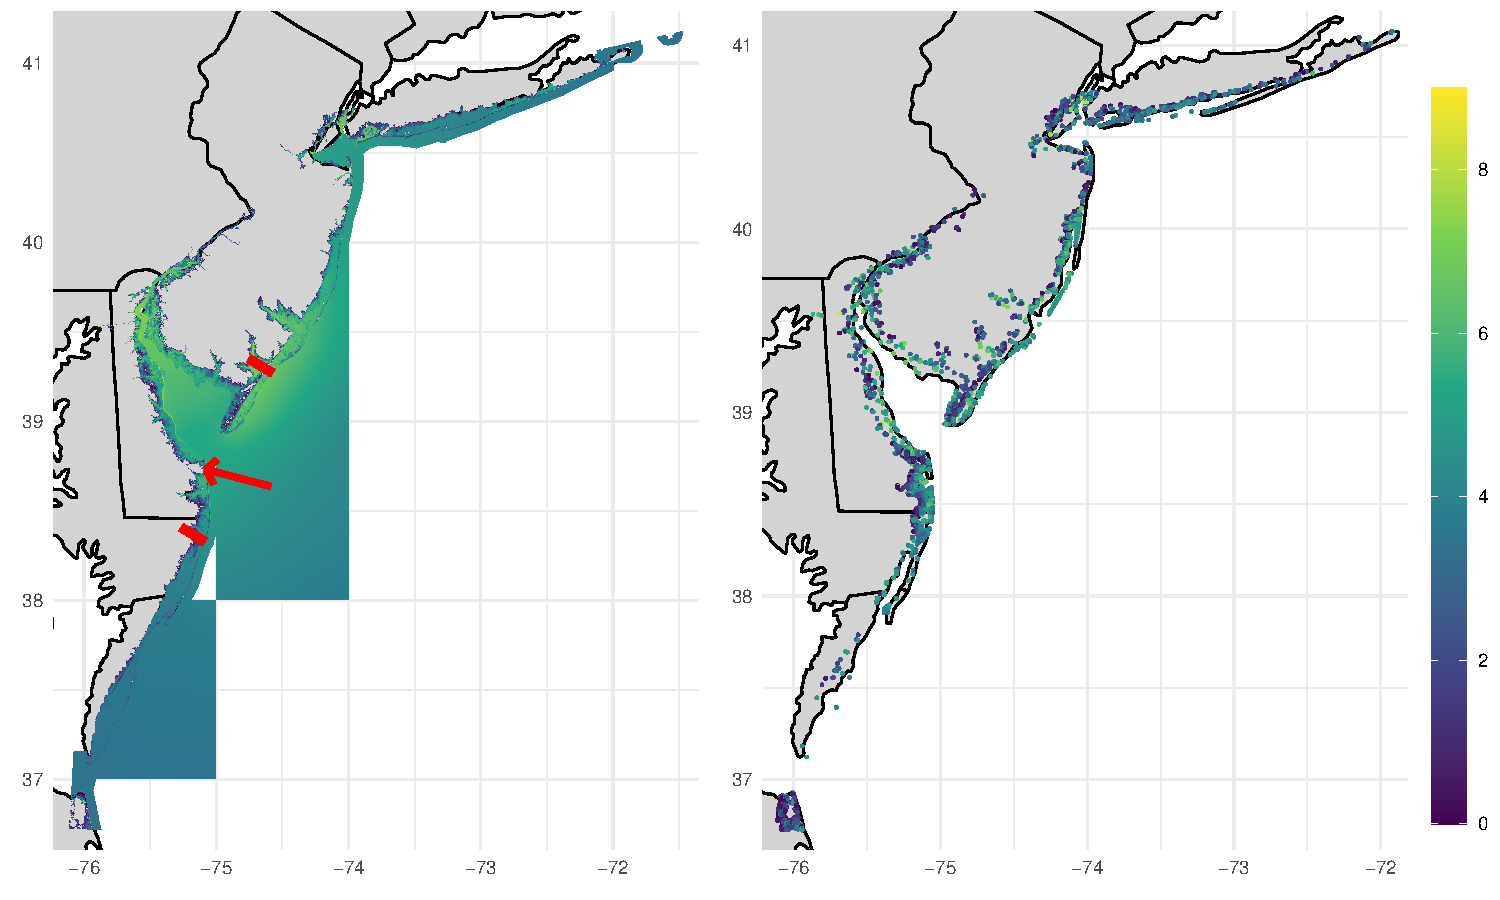
\includegraphics[height=\frametextheight]{./ch3/plots/slosh_combined}
    \end{center}
\end{frame} % SLOSH Locations

\note{
    \begin{itemize}
        \item SLOSH, or Sea, Lakes, and Overland Surge due to Hurricanes, is a storm-surge
            simulator.
        \item Based on 
    \end{itemize}
}

\begin{frame}
    \frametitle{Sea, Lakes, and Overland Surges due to Hurricanes (SLOSH)}
    \begin{minipage}{0.54\textwidth}
    {\footnotesize
    \begin{itemize}
        \item Simulations of storm surge given storm characteristics \par
        \begin{tabular}{cl}
            \textit{bearing}  & Direction (Angle) of storm eye at landfall \\
            \textit{velocity} & velocity of storm eye at landfall (kph)    \\
            \textit{latitude} & latitude of storm eye at landfall (dd)     \\
            \textit{pmin}     & Minimum atmospheric pressure of storm      \\
            \textit{pslr}     & Projected sea-level-rise over 100 years    \\
            \end{tabular}
        \item Each simulation an output grid
        \begin{itemize}
            \item \num{23119800} elements
            \item Spatial resolution 0.001 degrees, approx 90 meters.
        \item 4000 simulations
        \item Parameters sampled via Latin hypercube
        \end{itemize}
    \end{itemize}
    }
    \end{minipage}%
    ~
    \begin{minipage}{0.44\textwidth}
        {\footnotesize
        \begin{itemize}
            \item Intersect spatial grid with locations of interest
            \item Sort locations by type
            \item Create recursive subset \emph{slices} of data
            \begin{center}
            {\scriptsize
            % latex table generated in R 4.4.1 by xtable 1.8-4 package
% Thu Oct 10 21:07:30 2024
\begin{tabular}{lrrr}
  \hline
Dataset & Sites & Storms & $\text{P}(\bm{w}\not\leq \bm{b}_{q})$\\ 
  \hline
  Threshold  & \num{4414} & \num{1744} & \num{0.436} \\ 
  Delaware   & \num{950}  & \num{1253} & \num{0.313} \\ 
  Restricted & \num{65}   & \num{1092} & \num{0.273} \\ 
  Critical   & \num{12}   & \num{810}  & \num{0.202} \\ 
  \hline
\end{tabular}

            }
            \end{center}
            
            \vfill
            
            ~
        \end{itemize}
        
        }
    \end{minipage}
\end{frame} % SLOSH Intro

\note{
    \begin{itemize}
        \item
    \end{itemize}
}

\begin{frame}
    \frametitle{Identified Sites in Delaware}
    \begin{centering}
        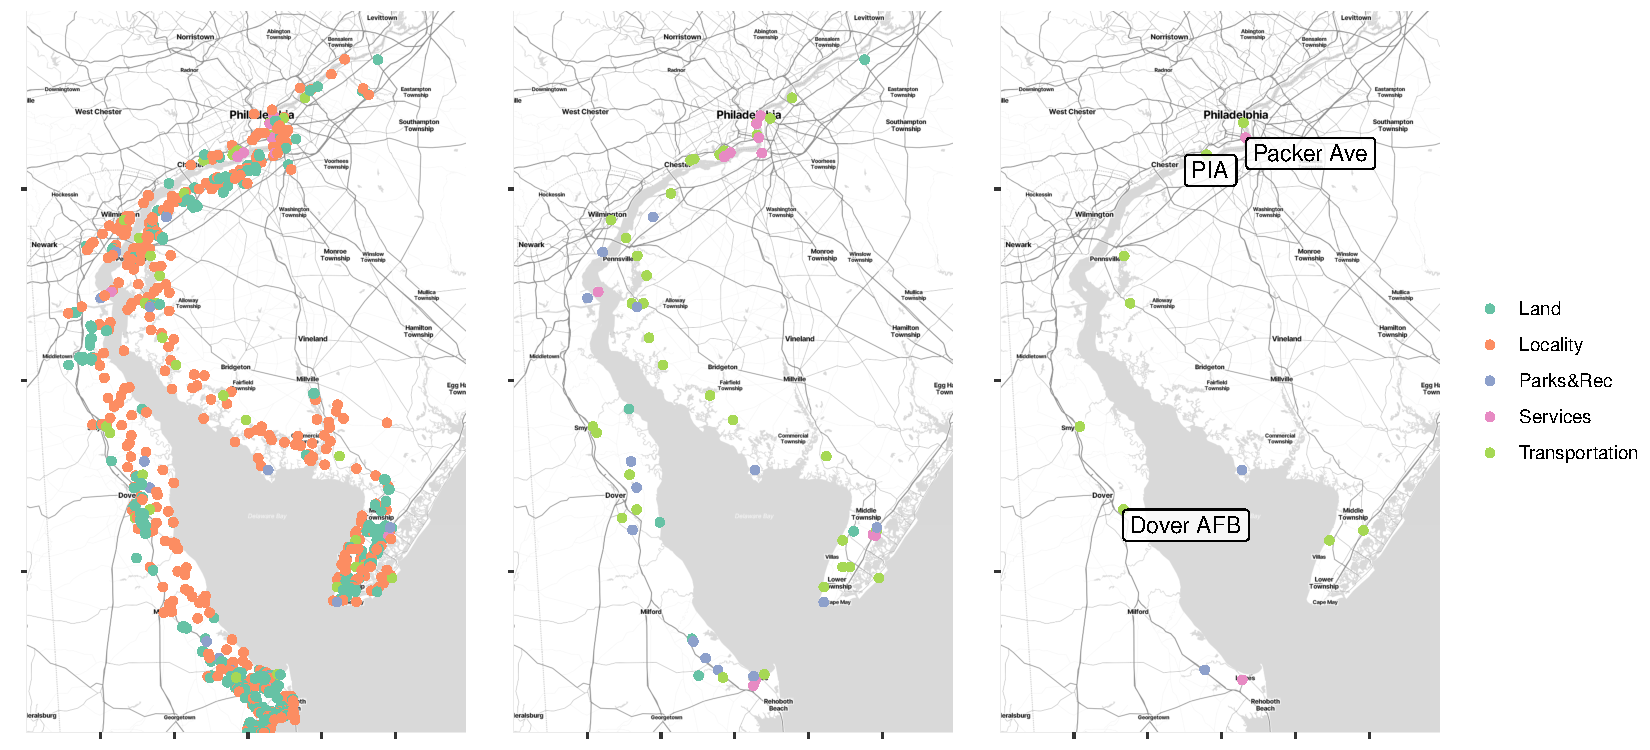
\includegraphics[width=0.99\linewidth]{./ch3/plots/delaware}
    \end{centering}
\end{frame} % Delaware Plot

\note{
    \begin{itemize}
        \item
    \end{itemize}
}

\begin{frame}
    \frametitle{Parameters of Surviving Storms}
    \begin{center}
        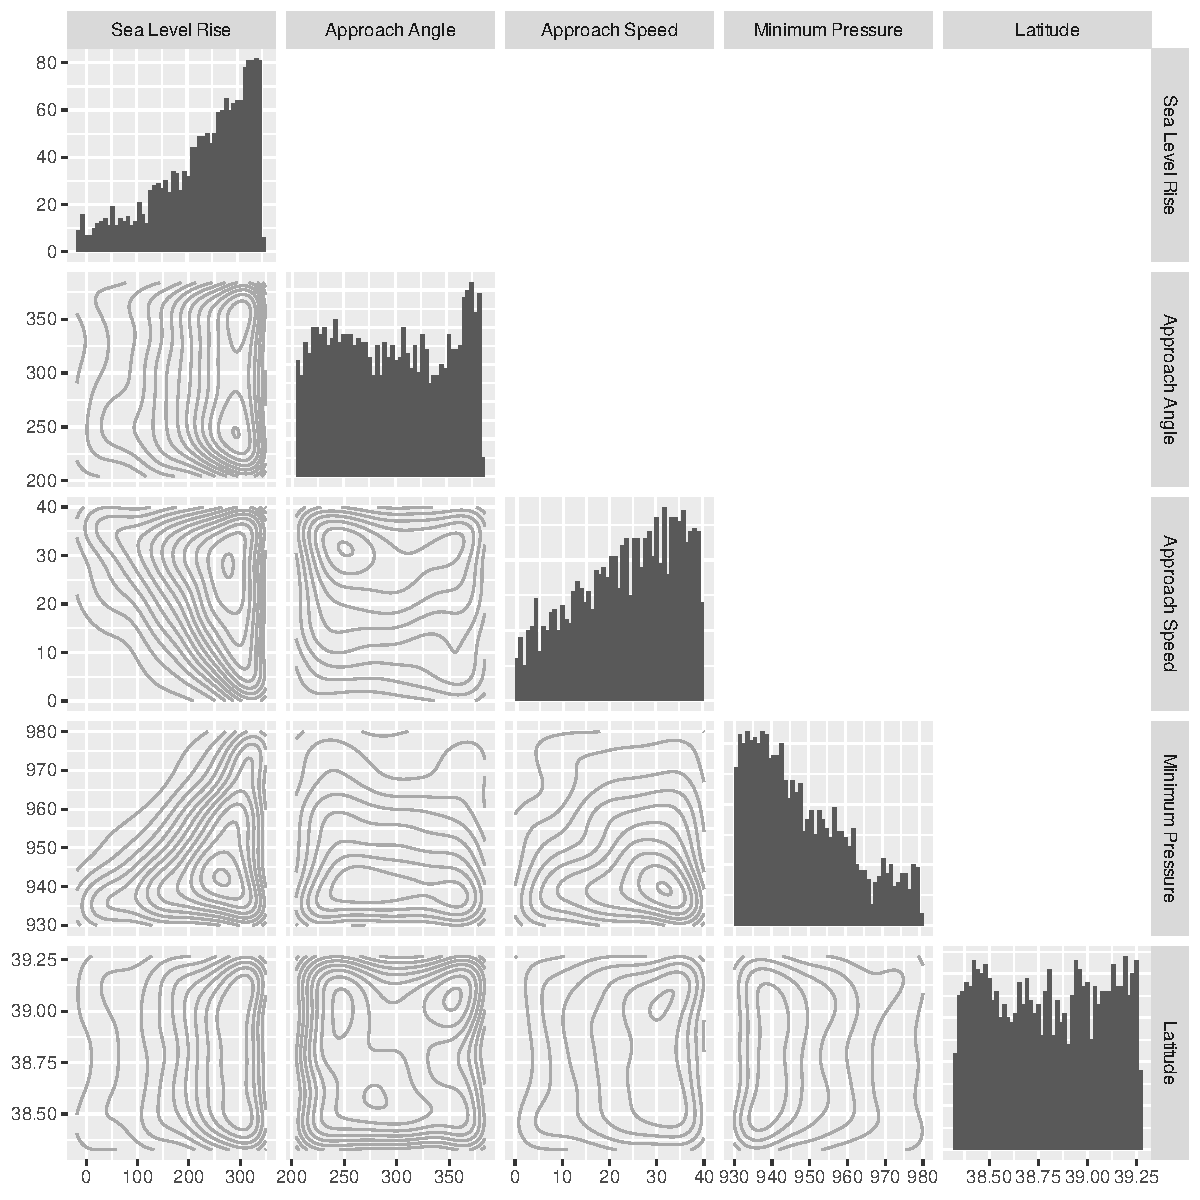
\includegraphics[height=0.99\frametextheight]{./ch3/plots/threshold_pairs}
    \end{center}
\end{frame} % Threshold Pairs

\note{
    \begin{itemize}
        \item
    \end{itemize}
}

\subsection{Methodology}

\begin{frame}
    \frametitle{Angular Data Model}
    {\small 
    \begin{itemize}
        \item The Model
        \[
        \begin{aligned}
                \bm{y}_n \mid \bm{\alpha}_n &\sim
                    \mathcal{PG}_p\left(\bm{Y}\mid\bm{\alpha}_n,\bm{1}\right)\\
                \bm{\alpha}_n &\sim G\\
                G &\sim \mathcal{PY}\left(\eta, \omega, G_0\right)        
            \end{aligned}
            ~\hspace{1cm}
            \begin{aligned}
                G_0 &= {\textstyle\prod}_{d = 1}^{D}
                    \text{Ga}(\alpha_{d}\mid \xi_{d},\tau_{d})\\
                \xi_{d} &\sim \mathcal{G}(\xi\mid a, b)\\
                \tau_{d} &\sim \mathcal{G}(\tau\mid c, d)
            \end{aligned}
        \]
        where $\omega \in [0,1)$ is discount parameter, $\eta > -\omega$ is concentration parameter.
    \item Fit via MCMC and (Mean Field) Variational Approximation
    \item MCMC Cluster Probability Full Conditional
        \[
        \mathbb{P}\left(\gamma_n = \jmath\mid \bm{y},\bm{\alpha},\bm{\rho}\right) = 
            \frac{\pi_\jmath\mathcal{PG}(\bm{y}_n\mid\bm{\alpha}_{\jmath})}{
                \sum_{k = 1}^J \pi_k\mathcal{PG}(\bm{y}_n\mid\bm{\alpha}_{\jmath})}
        \]
        where $\pi_{\jmath} = \rho_{\jmath}\prod_{k < \jmath}(1 - \rho_k)$
        \item MCMC Cluster Weight Full Conditional
        \[
        \rho_{\jmath}\mid\bm{\gamma} \sim 
            \mathcal{B}\left(\zeta_{\rho_\jmath 1} = 1 + C_{\jmath} - \omega,\; 
            \zeta_{\rho_{\jmath} 2} = {\textstyle \sum}_{k>\jmath} 
                C_k + \eta + \jmath \omega\right),
        \]
        where $C_\jmath = \sum_{n = 1}^N\bm{1}_{\gamma_n = \jmath}$.
    \end{itemize}
    }
\end{frame} % Angular Model

\subsubsection{Model Recovery}

\begin{frame}
    \frametitle{Marginally Assessing Model Fidelity}
    \begin{itemize}
        \item Comparative rise in energy score shrinks with data complexity
        \item How do we assess model fidelity then?
        \item Recovery of marginal CDF?
        \item Having sampled $\bm{V}^*$ from PPD, $R^*\sim\text{Pareto}(1)$, and $\bm{Z}^* = R^*\bm{V}^*$:
        \[
             W_d^* = \left[a_d\left(\frac{(Z_d^*)^{\xi_d} - 1}{\xi_d}\right) + b_d\right]_+
        \]
        where $\bm{\xi}$, $\bm{a}$, $\bm{b}$ were previously calculated.
    \end{itemize}
\end{frame} % Marginal Assessing Model Fidelity (Explanation)

\begin{frame}
    \frametitle{Marginal Recovery of CDF}
    \begin{center}
        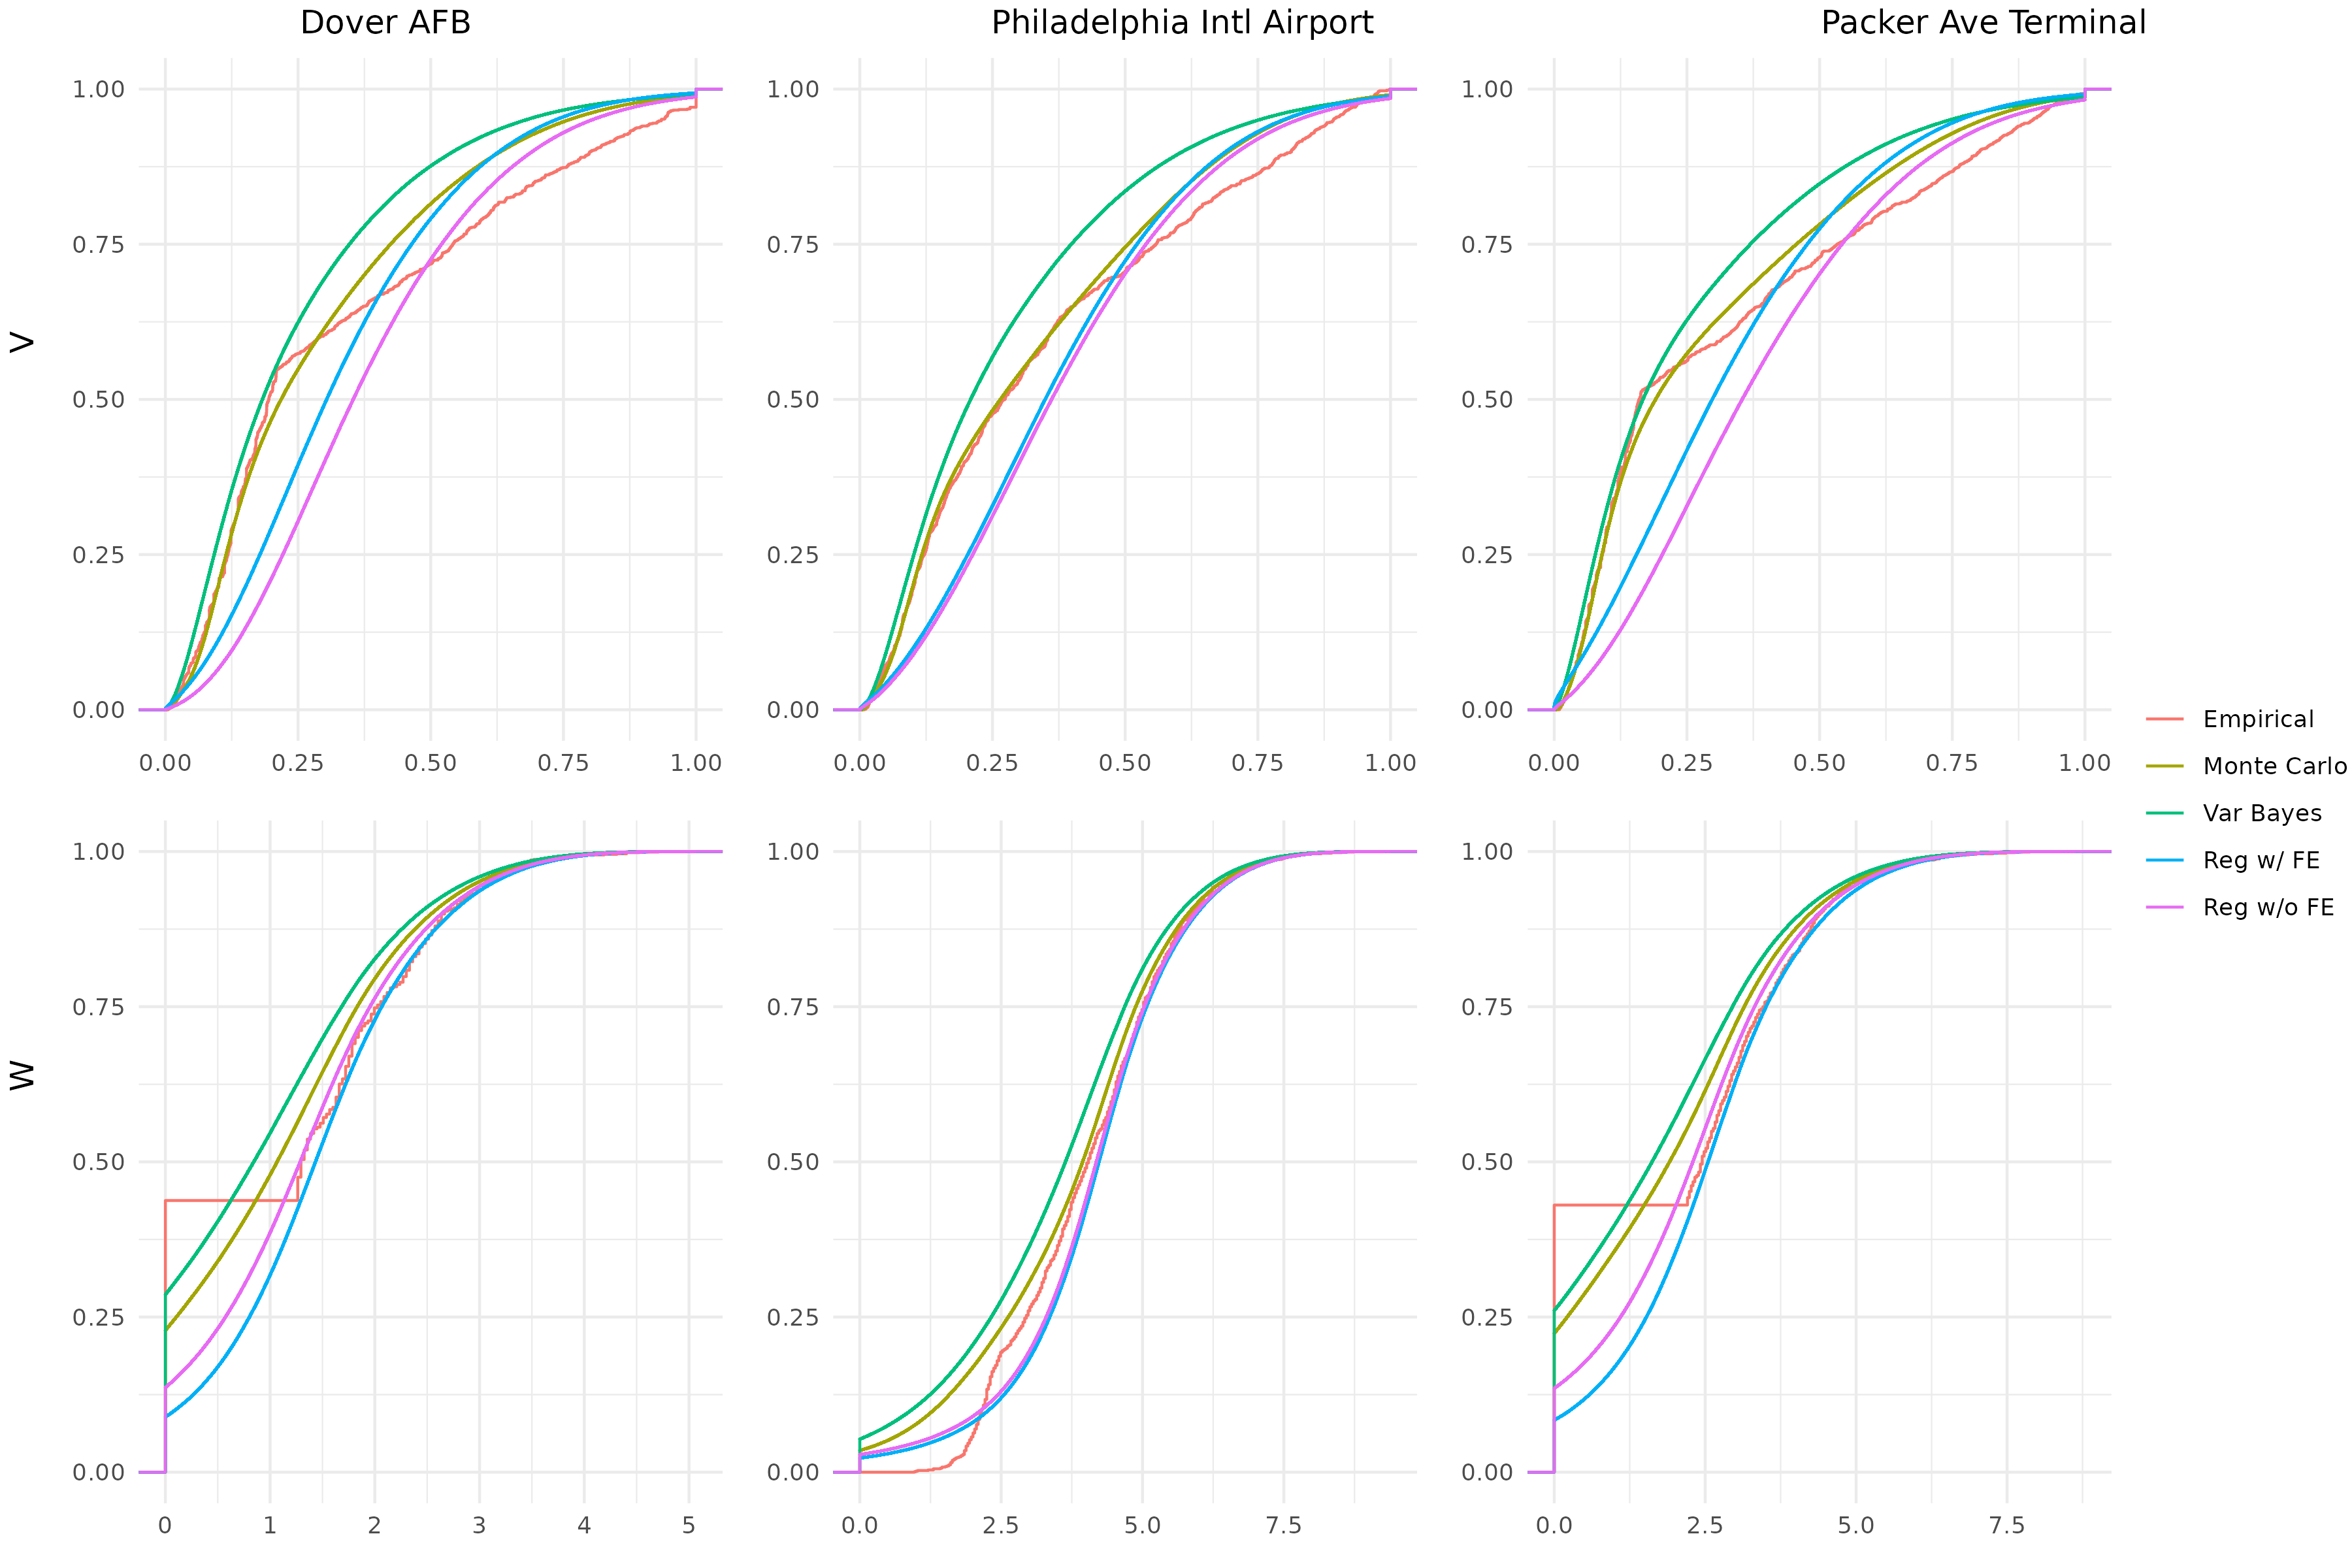
\includegraphics[height=0.99\frametextheight]{./ch3/plots/delaware_marginal_cdfs}
    \end{center}
\end{frame} % Marginal Recovery of CDF (Plot)

\begin{frame}
    \frametitle{Extant Clusters}
    \begin{center}
        % latex table generated in R 4.4.1 by xtable 1.8-4 package
% Thu Oct 10 16:54:40 2024
\begin{tabular}{lrrrr}
  \hline
Slice & Var Bayes & Monte Carlo & Reg w/o RE & Reg w/ RE \\ 
  \hline
  Threshold & 3 & 37 & ~ & ~ \\ 
  Delaware & 4 & 30 & ~ & ~ \\ 
  Restricted & 8 & 21 & 127 & 118 \\ 
  Critical & 11 & 51 & 30 & 22 \\ 
  \hline
\end{tabular}

    \end{center}
    {\footnotesize Counts of emergent clusters identified in data slices via posterior sampling.}
\end{frame} % Extant Clusters

\subsubsection{Conditional Survival Probability}

\begin{frame}
    \frametitle{Conditional Survival Curves}
    \begin{prop}
      For $\alpha \subset \lbrace 1, \ldots, D\rbrace$
    \[
        \mathbb{P}\left[\bigcap_{d\in\alpha}Z_{d} > z_d\mid \bigcap_{d\not\in\alpha}\bm{Z}_{d} > \bm{z}_{d}\right] =
        \frac{\mathbb{E}\left[\bigwedge_{d = 1}^D \frac{V_k}{z_k}\right]}{
                      \mathbb{E}\left[\bigwedge_{d\not\in\alpha}\frac{V_d}{z_d}\right]}
    \]
      where $\bm{V} = \bm{Z}\,/\,\lVert\bm{Z}\rVert_{\infty}$.
  \end{prop}
    \begin{itemize}
        \item Conditioning on the state of the field
        \item $\bm{w}_n$, $\bm{v}_n$ is maximum surge at each location during storm $n$---not simultaneous
        \item We can use $\bm{Z}_{\neg\alpha}$ to specify \emph{scenarios}
    \end{itemize}
\end{frame} % Conditional Survival Probability

\begin{frame}
    \frametitle{Conditional Survival Curves}
    \begin{center}
        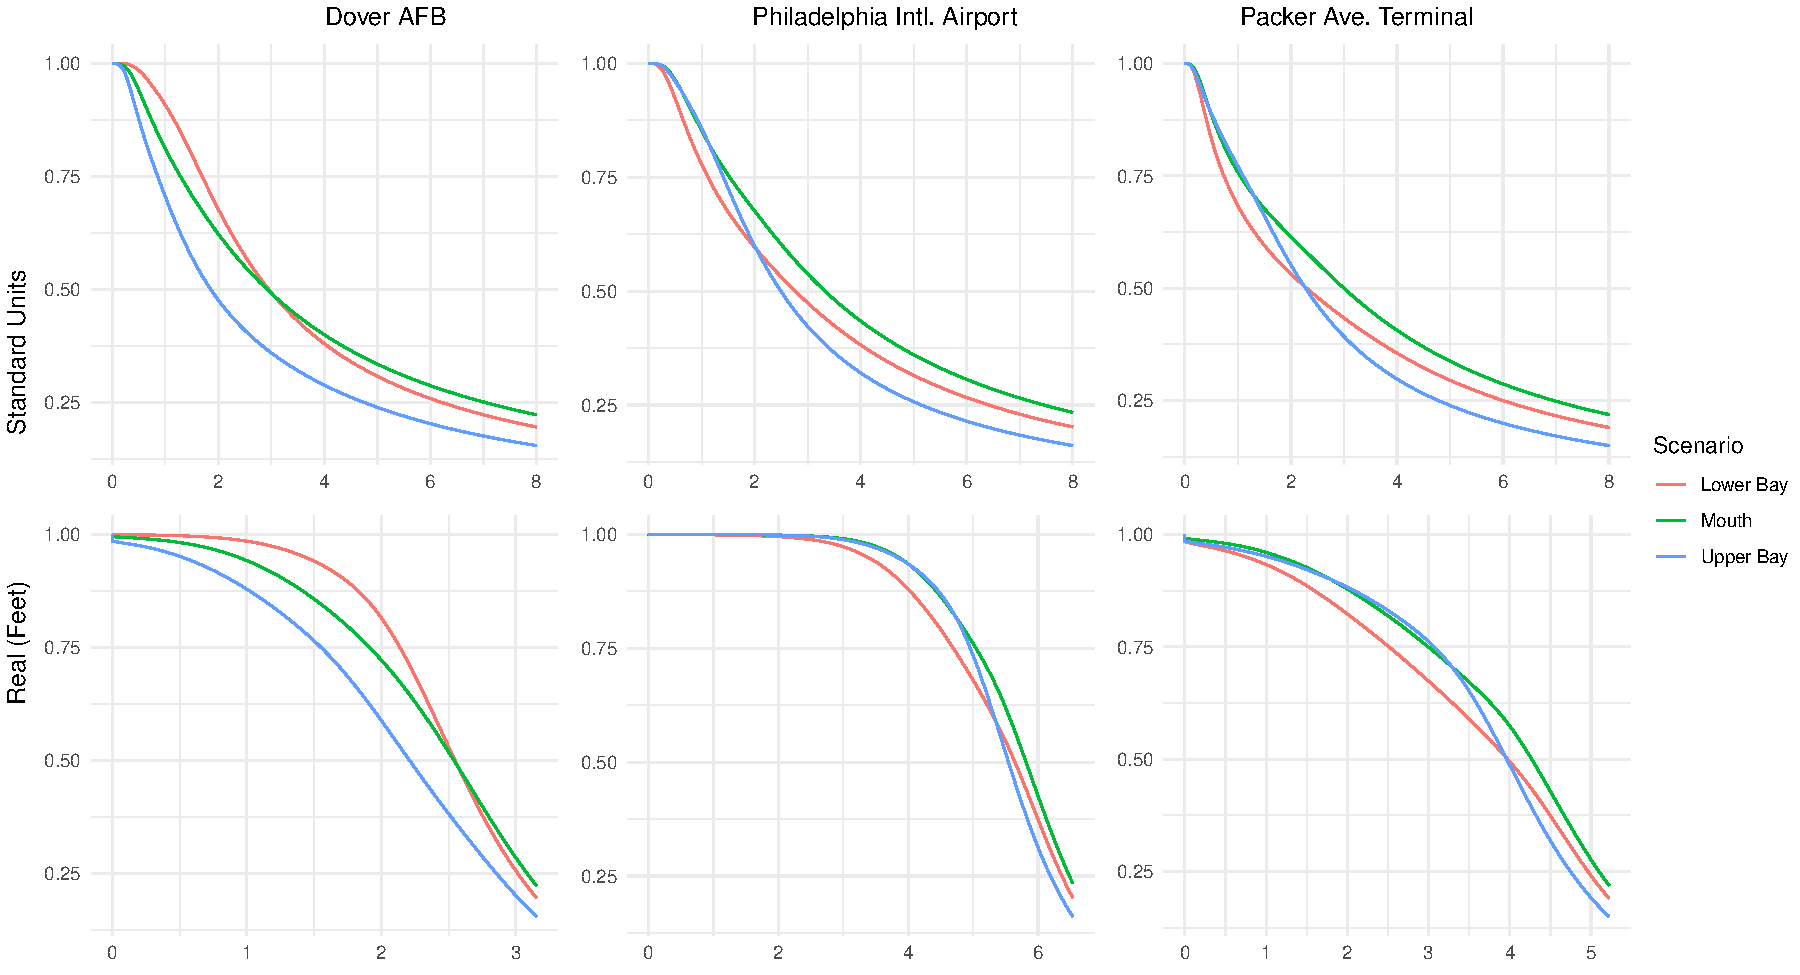
\includegraphics[height=0.99\frametextheight]{./ch3/plots/condsurv/condsurv_1d_mcmc_combined}
    \end{center}
\end{frame} % Conditional Survivla

\begin{frame}
    \frametitle{Conditional Survival Surfaces}
    \begin{center}
        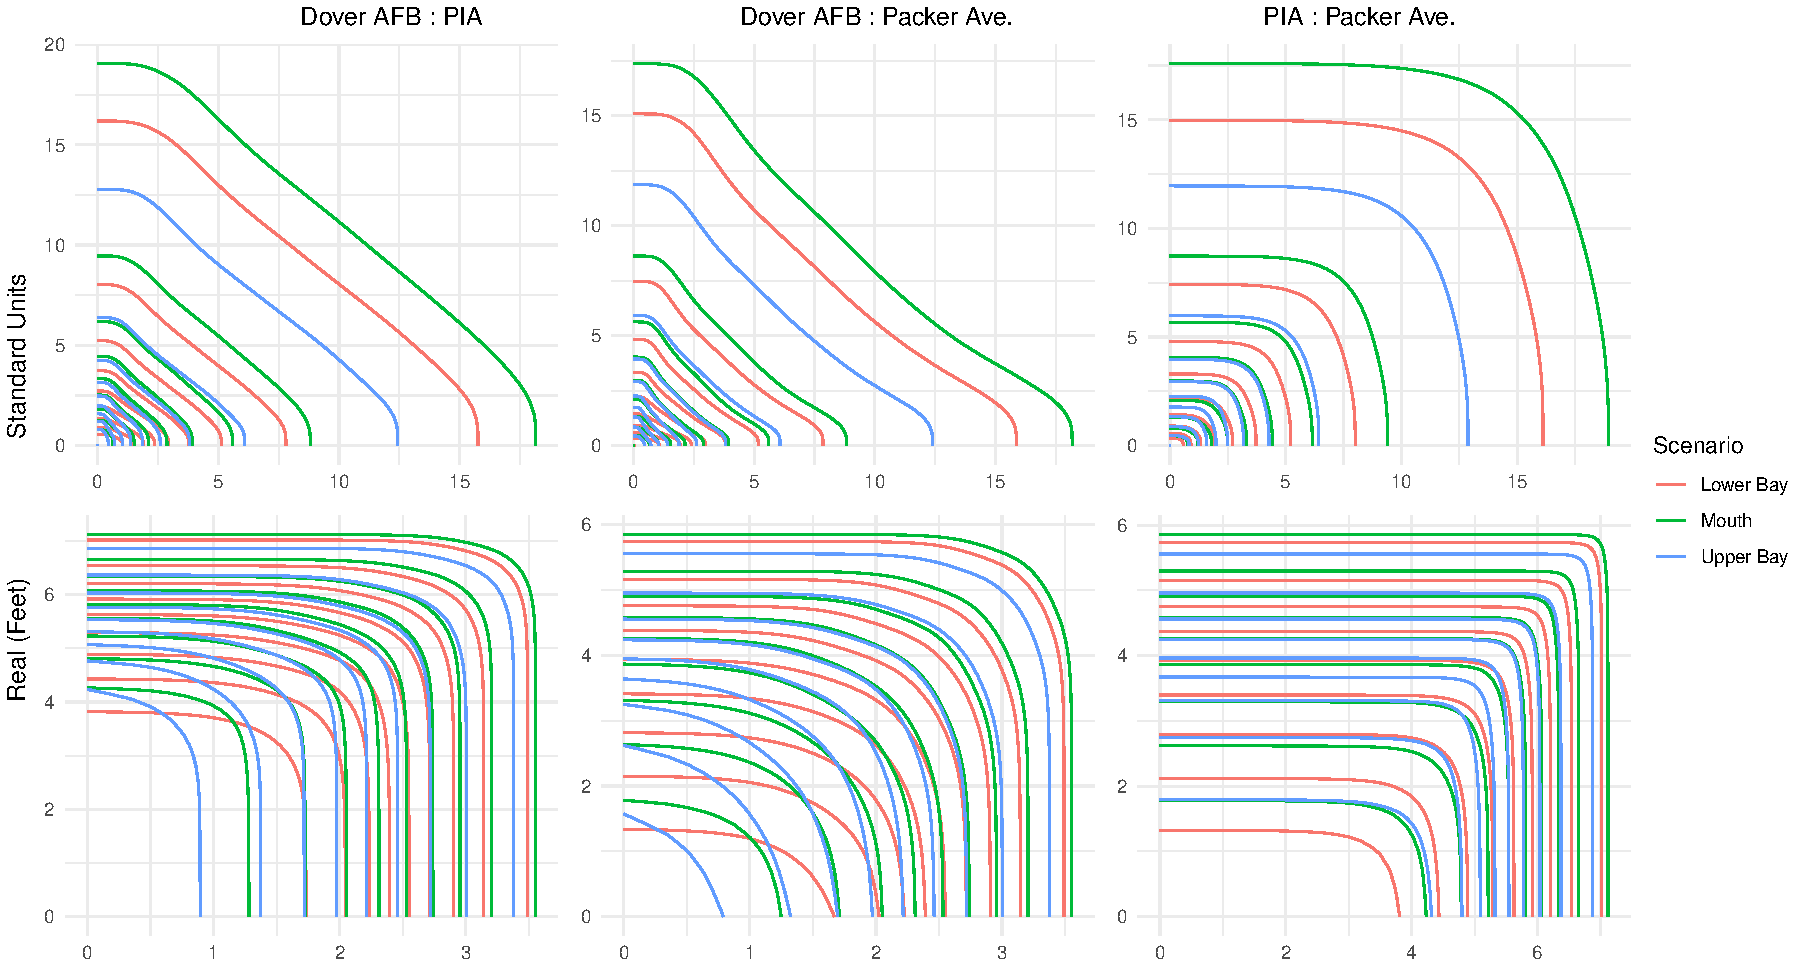
\includegraphics[height=0.99\frametextheight]{./ch3/plots/condsurv/condsurv_2d_mcmc_combined}
    \end{center}
\end{frame} % Conditional Survival Surfaces

\subsection{Regression}

\begin{frame}
    \frametitle{Regression Model}
    {\footnotesize 
    \begin{itemize}
        \item Consider
        \[
            \bm{y}_n \sim \mathcal{PG}(\bm{y}\mid g(\bm{x}_n^T\bm{\theta}), \bm{1});
            \hspace{1cm}
            g(\cdot) = \log[1 + \exp(\cdot)]
        \]
        Some discussion necessary as to the dimensionality of $\bm{\theta}$.
        \item $\bm{x}_n$ of dimension $L$
        \item A \emph{fully specified} model has, for each dimension $d$, a vector $\bm{\theta}_{nd}$ of dimension $L$.
        \[
        \bm{y}_n \sim \int_0^{\infty}
            \prod_{d = 1}^D \mathcal{G}\left(r_ny_{nd}\mid 
                g(\bm{x}_n^T\bm{\theta}_{nd}), 1\right) \times J^{\neg r}(\bm{y}_n) r^{D-1}\text{d}r 
        \]
        %\pause
        or, more succinctly
        \[
        \bm{y}_n \sim \mathcal{PG}\left(\bm{y}_n \mid g((\bm{x}_n 
            \otimes \bm{I}_{D})^T\bm{\theta}), \bm{1}\right)
        \]
        where $\otimes$ is Kronecker Product.
        \item A Regression Model
        \[
        \begin{aligned}
            \bm{y}_n &\sim \mathcal{PG}\left(\bm{y}\mid 
                g\left((\bm{x}_n\otimes\bm{I}_D)^T\bm{\theta}_n\right), \bm{1}\right)\\
            \theta_n &\sim G\\
            G &\sim \mathcal{PY}(G\mid\eta, \omega, G_0)
        \end{aligned}
        ~\hspace{2cm}
        \begin{aligned}
            G_0 &= \mathcal{N}(\bm{\theta} \mid \mu, \Sigma)\\
            \Sigma &\sim \mathcal{IW}(\Sigma\mid \nu, \psi)\\
            \mu\mid\Sigma &\sim \mathcal{N}(\mu\mid \bm{0}, \Sigma / \kappa)
        \end{aligned}
        \]
    \end{itemize}
    }
\end{frame} % Regression Model (Fully Specified)

\begin{frame}
    \frametitle{Fully Specified Model Recovery}
    % \begin{center}
    % 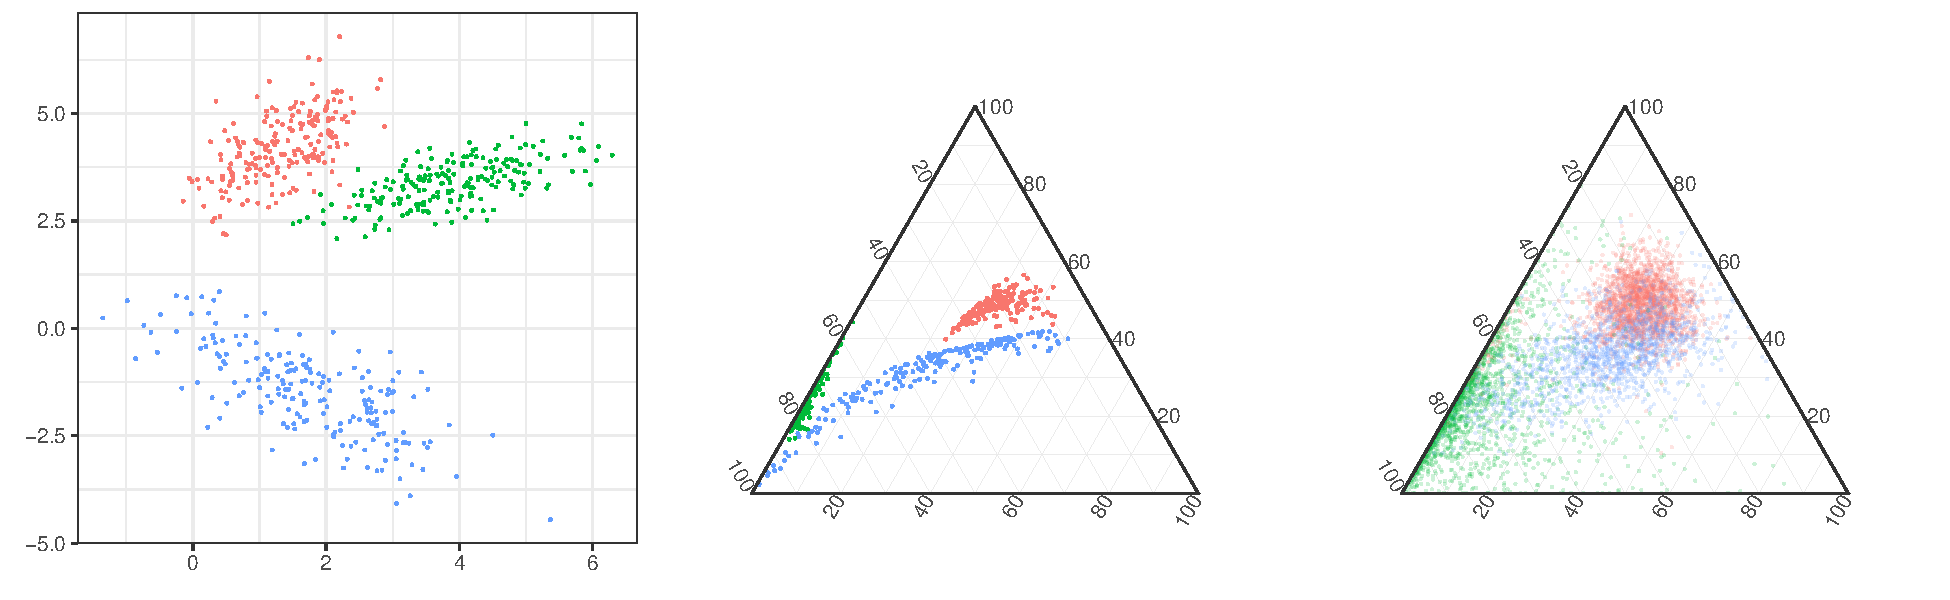
\includegraphics[width = \textwidth]{./ch3/plots/simulated_reg}
    % \end{center}
    % \begin{center}
    % {\scriptsize
    % (Left) $\bm{x}$ - Inputs\hspace{1cm}(Middle) $\bm{y}$ - Outputs\hspace{1cm} (Right) $\bm{y}^*$ Posterior Predictive Sample
    % }
    % \end{center}
    \begin{figure}[h]
    \centering
    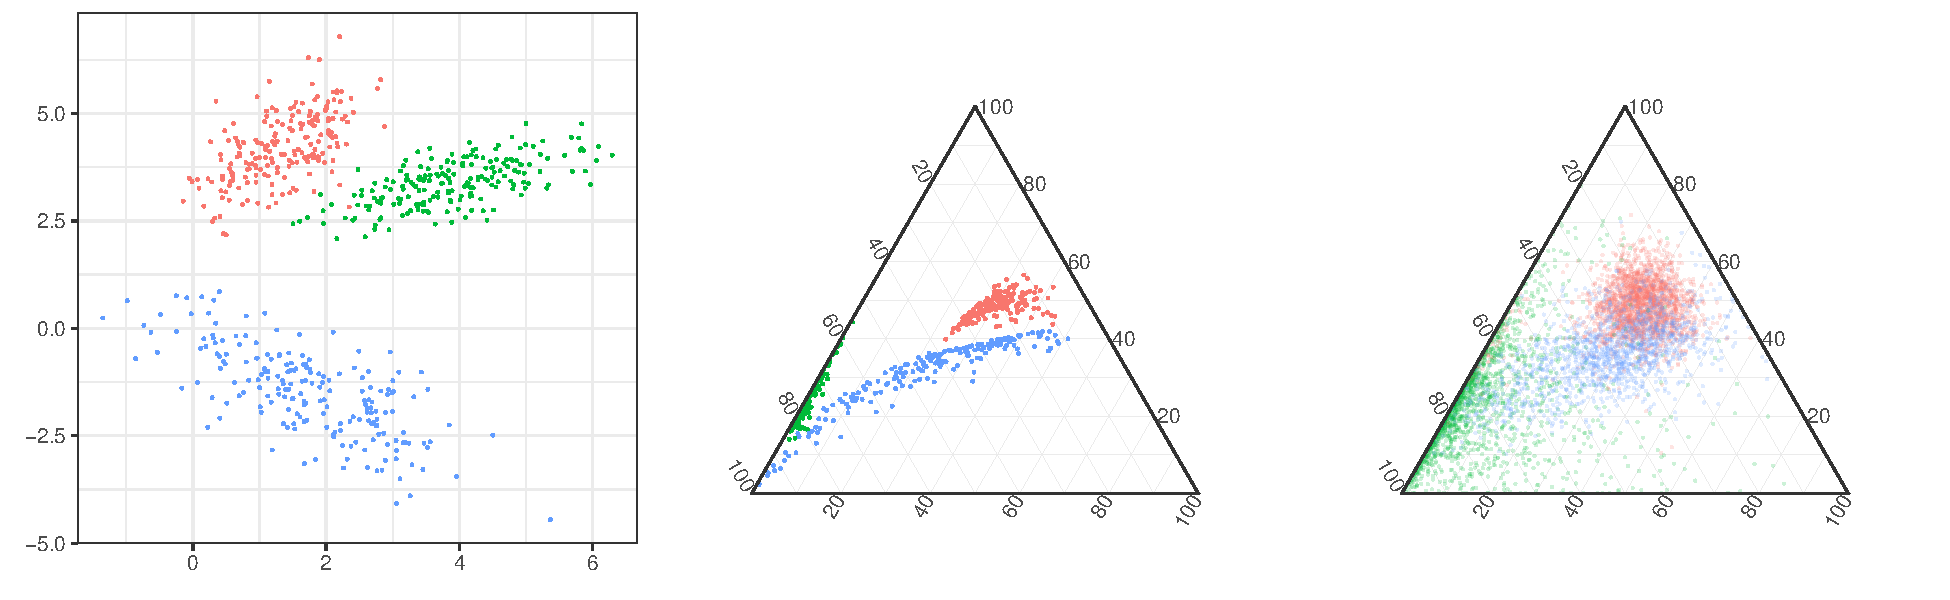
\includegraphics[width=\textwidth]{./ch3/plots/simulated_reg}
    \caption{(Left) Regressors; (Middle) Output; (Right) Posterior Predictive Sample.
        Cluster labels are \emph{recovered}.
        }
    \end{figure}
\end{frame} % Fully Specified Model Recovery

\begin{frame}
    \frametitle{A More Sensible Model}
    \begin{itemize}
        \item Overload $\bm{x}_{nd}$, the parameters of observation $n$ at location $d$ as
        \begin{description}
            \item[$\bm{x}_{n,\text{obs}}$] Parameters of $n$th storm (scaled)
            \item[$\bm{x}_{d,\text{loc}}$] Information pertaining to $d$th location 
                (lat., lon., elevation)
            \item[$\bm{x}_{nd,\text{int}}$] Any interaction thereof---Currently 
                distance to eye at landfall (hectomiles).
        \end{description}
        \item Then $\bm{\theta}$ has dimensionality $5 + 3 + 1 = 9$
        \item Location random effect $\varepsilon_d$
        \item The Model:
        \[
            \bm{y}_n \sim \mathcal{PG}\left(\bm{y}\mid g(\bm{x}_n^T\bm{\theta}_n 
                + \bm{\varepsilon}), \bm{1}\right)
            \hspace{1.5cm}
            \varepsilon_d \sim \mathcal{N}\left(\varepsilon\mid 0, 
                \sigma_{\varepsilon}^2\right)
        \]
        \item Model fitted via MCMC.
    \end{itemize}
\end{frame} % SLOSH Regression Model

\subsubsection{Conditional Survival Probability (Regression Style)}

\begin{frame}
    \frametitle{Conditional Survival Curves}
    \begin{center}
        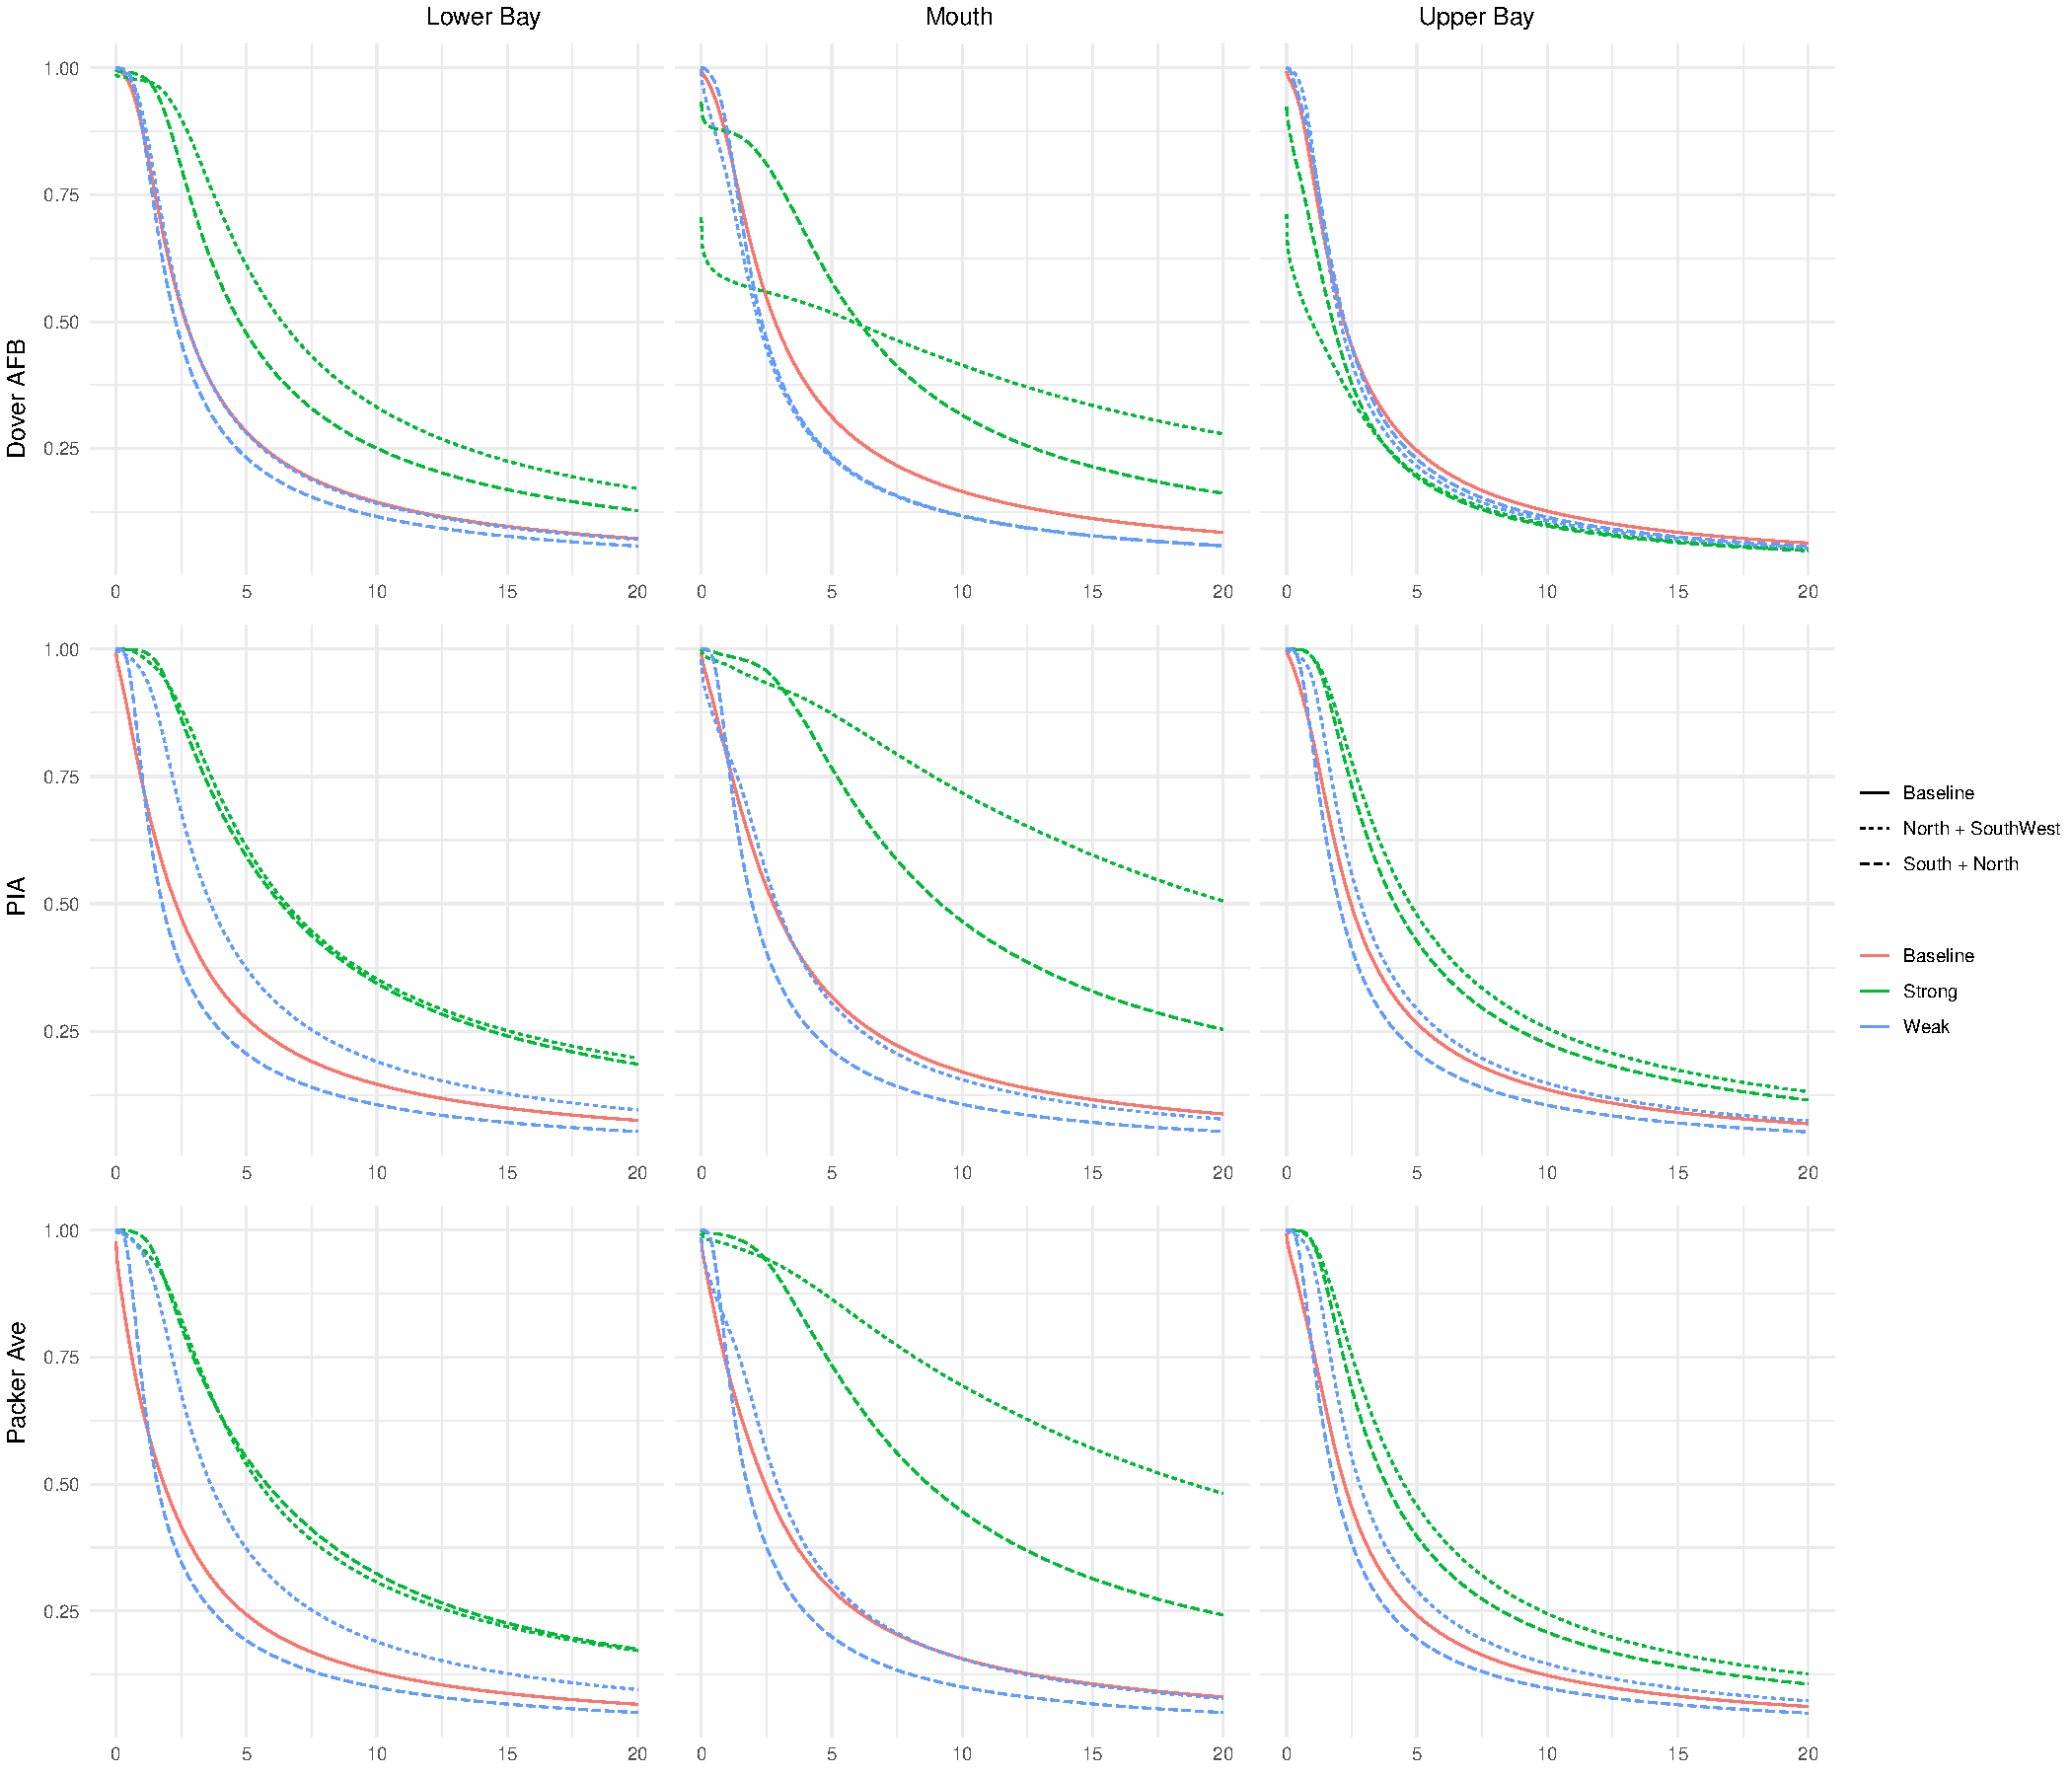
\includegraphics[height=0.99\frametextheight]{./ch3/plots/condsurv_reg/condsurv_reg_1d_std}
    \end{center}
\end{frame}

\subsection{Conclusion}

\section{Conclusion}

\subsection{Summary}

\begin{frame}
    \frametitle{BNP Inference for Multivariate PoT Models}
    \begin{itemize}
        \item Separation of inference for angular and radial components of extreme vector
        \item Model selection using energy score, with a novel negative definite kernel
        \item Introduced projected gamma distribution as an angular distribution
        \item Used projected gamma as the kernel of a BNP mixture angular data model
        \item Infer the dependence structure of geographical regions in IVT
    \end{itemize}
\end{frame}

\begin{frame}
    \frametitle{Anomaly Detection in PoT Settings and Angular Representations of Categorical Data}
    \begin{itemize}
        \item Separation of angular and radial anomaly scores for extreme data
        \item Angular anomaly scores based on posterior-predictive density
        \item A categorical data model
        \begin{itemize}
            \item Angular representation of categorical data
            \item Novelty scores based on said angular representation
        \end{itemize}
        \item A \emph{mixed} data model
        \begin{itemize}
            \item Novelty scores---independent or combined regimes
        \end{itemize}
        \item Scores are performant on canonical datasets relative to canonical methods
        \begin{itemize}
            \item Dependent on the concentration of \emph{anomalous} events in training data---less is better
        \end{itemize}
    \end{itemize}
\end{frame}

\begin{frame}
    \frametitle{Extremal Dependence of Storm Surge Using a PoT Model}
    \begin{itemize}
        \item Application of BNP mixture of projected gammas at scale
        \item Inferred dependence structure of extreme storm surge simulations under SLOSH
        \item Conditional survival probability functions given various scenarios
        \item Angular regression model using projected gamma distribution
        \item Expand conditional survival analysis to consider storm characteristics
    \end{itemize}
\end{frame}

\subsection{Looking Forward}

\begin{frame}
    \frametitle{Problems and Solutions}
    \begin{description}
        \item[Problems]~ 
            \begin{itemize}
                \item Edge-seeking behavior of gamma family
                \item Convergence towards a single cluster with $\bm{\alpha}_{\jmath} \to \bm{0}$
                \item Mean Field Variational Bayes inadequate for BNP mixture weights
            \end{itemize}
        \item[Solutions]~
            \begin{itemize}
                \item Variational-within-Gibbs approach \cite{Loaizamaya2022}
                \begin{itemize}
                    \item Gibbs-sampling stick-breaking weights, cluster ID's
                    \item VI for cluster parameters
                \end{itemize}
                \item Conditioning the transformation on 
                    $\argmax\limits_{d \in \lbrace 1,\ldots, D\rbrace} Z_d$
                \item Restricting cluster shapes such that $\vee_{d = 1}^D\; \alpha_d > 1$
                \item Zero-inflated / Sparse Projected Gamma
            \end{itemize}
    \end{description}
\end{frame}

\begin{frame}[plain]
    \begin{center}
        
\includegraphics[height=0.7\frametextheight]{./ch1/images/fin}
    \end{center}
\end{frame} % Fin 

\appendix

\begin{frame}[allowframebreaks]
    \frametitle{References}
    \footnotesize
    \bibliography{./refs}
\end{frame}

\section*{Appendix}

\subsection*{Simulation Study Details}

\begin{frame}
    \label{pgpareto:simstudydetails}
    \frametitle{Simulation Study}
    \begin{itemize}
        \item Finite mixture of Gammas
        \item For each Number of Mixture Components (3,6,9,12):
            \begin{itemize}
                \item Generate a data-set of 20 columns
                \item output subsets of $D = 3,6,12,20$ columns projected 
                    onto $\mathcal{S}_{\infty}^{D-1}$.
                \item Cross-Validated:
                    \begin{itemize}
                        \item Fit angular data models to projected data
                        \item Calculate average energy score of posterior 
                            predictive against out-of-sample set.
                    \end{itemize}
            \end{itemize}
    \end{itemize}
    \hyperlink{pgpareto:simstudy}{\beamerbutton{Simulation Study Results}}
\end{frame} % Simulation Study Details

\subsection*{Projection onto $\mathcal{S}_p^{d-1}$}

\begin{frame}
  \frametitle{Jacobian}
  \label{pgpareto:jacobian}
  \begin{equation*}
    \begin{bmatrix}
      y_1 & r & 0 & \ldots & 0\\
      y_2 & 0 & r & \ldots & 0\\
      \vdots & \vdots & \vdots & \ddots & \vdots\\
      y_{D-1} & 0 & \ldots & 0 & r \\
      \left(1 - {\scriptsize\sum_{d=1}^{D-1}}y_d^p\right)^{\frac{1}{p}} &
        - ry_1^{p-1}\phi & -ry_2^{p-1}\phi & \cdots & -ry_{D-1}\phi
    \end{bmatrix}
  \end{equation*}
  where $\phi = \left(1 - {\scriptsize\sum_{d=1}^{D-1}}y_d^p\right)^{\frac{1}{p} - 1}$
  %\pause
  \begin{equation*}
  \lvert J \rvert = r^{d-1}\left[\left(1 - {\textstyle\sum}_{d = 1}^{D-1}y_d^p\right)^{\frac{1}{p}} +
      {\textstyle\sum}_{d = 1}^{D-1}y_d^p\left(1 - {\textstyle\sum}_{d=1}^{D-1}
          y_d^p\right)^{\frac{1}{p} - 1}\right]
  \end{equation*}
\end{frame} % Unit Sphere - Jacobian

\subsection*{Projected Gamma Inference}

\begin{frame}
    \frametitle{Data Augmentation and Inference}
    \label{pgpareto:projgammainference}
    {\small 
    \begin{itemize}
        \item Sample $r\mid\bm{\alpha},\bm{\beta},\bm{y}$
        \[
            r\mid\bm{\alpha},\bm{\beta},\bm{y} \sim 
                \text{Ga}\left(r\mid \sum_{d = 1}^D \alpha_d, 
                    \sum_{d = 1}^D\beta_dy_d\right)
        \]
        %\pause
        \item Given $r$, the Likelihood
        \[
        L(\bm{\alpha},\bm{\beta}\mid \bm{r},\bm{y}) 
            \propto \prod_{n = 1}^N\prod_{d = 1}^D
            \text{Ga}\left(r_ny_{nd}\mid\alpha_d,\beta_d\right),
        \]
        %\pause
        becomes separable by dimension.
        \[
        L(\alpha_d,\beta_d) \propto 
            \prod_{n = 1}^N\text{Ga}\left(r_ny_{nd}\mid\alpha_d,\beta_d\right)
        \]
        %\pause
        \item With appropriate choice of prior, inference can be parallelized.
    \end{itemize}
    }
    \hyperlink{pgpareto:projectedgamma}{\beamerbutton{Projected Gamma}}
\end{frame} % Data Augmentation and Inference


\begin{frame}
  \frametitle{Projected Gamma Model - Inference}
  \label{pgpareto:pginference}
  \begin{itemize}
    \item Full conditional for $\beta_d$
      \begin{equation*}
        \beta_d\mid \bm{ y}, r, \alpha_d \sim \text{Ga}\left(n\alpha_d + \zeta_d,
                {\textstyle \sum}_{n = 1}^Nr_ny_{nd} + \sigma_d\right)
      \end{equation*}
    %\pause
    \item Posterior for $\alpha_d$
      \begin{equation*}
        f(\alpha_d \mid \bm{ y}, r) \propto
          \frac{\left({\textstyle \prod}_{n = 1}^Nr_ny_{nd}\right)^{\alpha_d - 1}}{
            \Gamma^N(\alpha_d)} \times \alpha_d^{\xi_d - 1}\exp\{-\tau_d\alpha_d\} \times
            \frac{\Gamma(N\alpha_d + \zeta_d)}{
            \left({\textstyle\sum}_{n = 1}^N r_ny_{nd} + \sigma_d
                  \right)^{(N\alpha_d + \zeta_d)}}
      \end{equation*}
    %\pause
    \item If $\beta_d = 1$, then
    \begin{equation*}
      f(\alpha_d \mid \bm{ y}, r) \propto
        \frac{\left({\textstyle\prod}_{n = 1}^N r_ny_{nd}\right)^{\alpha_d - 1}}{\Gamma^N(\alpha_d)} \times
        \alpha_d^{\xi_d - 1}\exp\{-\tau_d\alpha_d\}
    \end{equation*}
  \end{itemize}
  \hyperlink{pgpareto:angulardatamodel}{\beamerbutton{Angular Data Model}}
\end{frame}

\subsection*{Negative Definite Kernel}

\begin{frame}
    \frametitle{Not Geodesic Distance}
    \label{pgpareto:notgeodesic}
    \begin{itemize}
        \item Geodesic distance is length of shortest path from points $\bm{a}$ to $\bm{b}$.
        \item $\mathbb{S}_1^{D-1}$ easy.  $\mathbb{S}_2^{D-1}$ more difficult. 
            No simple closed form for $\mathbb{S}_{\infty}^{D-1}$
        \item $\mathbb{S}_{\infty}^{D-1}$ easier\ldots and harder.
        \begin{itemize}
            \item All faces are pairwise adjacent.
            \item A \emph{net} is an unfolding of a geometric figure.  
            \item Shortest path corresponds to straight line on appropriate net.
            \item $D!$ possible nets.  But $\sum_{d = 1}^{D-2}\binom{D-2}{d}$ 
                possible distinct paths.  Still too much.
        \end{itemize}
    \end{itemize}
    \hyperlink{pgpareto:energyscore}{\beamerbutton{Energy Score}}
\end{frame} % Not geodesic distance 

\begin{frame}
    \frametitle{Upper Bound on Geodesic Distance on $\mathbb{S}_{\infty}^{D-1}$}
    \label{pgpareto:kerneldetails}
    \begin{itemize}
        \item Let $\mathbb{C}_e^{D-1} = \left\lbrace\bm{v} : \bm{v} \in 
            \mathbb{S}_{\infty}^{D-1},\;\bm{v}_e = 1\right\rbrace$.
        %\pause
        \item Let $\bm{a}\in \mathbb{C}_d^{D-1}$, $\bm{b}\in\mathbb{C}_e^{D-1}$, and
            $\mathbb{C}_{de}^{D-2} = \mathbb{C}_d^{D-1}\cap \mathbb{C}_e^{D-1}$
            for $d,e\in \lbrace 1,\ldots,D\rbrace$.
            \[
            g(\bm{a},\bm{b}) = \begin{cases}
                \min\limits_{\bm{c}\in\mathbb{C}_{de}^{D-2}}\lVert \bm{c} - \bm{a}\rVert_2 + 
                    \lVert \bm{b} - \bm{c}\rVert_2 &\text{ for }d\neq e\\
            \lVert \bm{a} - \bm{b}\rVert_2 &\text{ otherwise}
            \end{cases}
            \]
        %\pause
        \item A Computationally Efficient Form
        \[
            g(\bm{a},\bm{b}) = \lVert \bm{a} - \bm{b}^{\prime}\lVert_2 
            \text{ where }\bm{b}^{\prime} = \begin{cases}
                b_i &\text{ for }i\neq d,e\\
                1 &\text{ for }i = d\\
                2 - b_d &\text{ for }i = e
                \end{cases}
        \]
        \item Thus, a valid negative definite kernel and distance analogue on $\mathbb{S}_{\infty}^{D-1}$.
    \end{itemize}
    \hyperlink{pgpareto:energyscore}{\beamerbutton{Energy Score}}
\end{frame} % Upper bound on geodesic distance 

\begin{frame}
    \frametitle{Negative Definite Kernel - Proof}
    \label{pgpareto:negdefkernel}
    \begin{itemize}
        \item In the first case, where $\bm{a}$ and $\bm{b}$ $\rightarrow$ Euclidean distance. 
        \item In the second case, $\bm{a}$ and $\bm{b}$ reside on separate
  faces.  
  \begin{itemize}
      \item $c$ is unique, $\lVert\bm{c} - \bm{a}\rVert_2 = \lVert\bm{a} - \bm{c}\rVert_2$ $\rightarrow$ symmetry in the arguments.
      \item Then for the other property of negative definiteness
  \begin{equation*}
    \begin{aligned}
      \sum_{i = 1}^N\sum_{j = 1}^N \alpha_i\alpha_j g(\bm{x}_1,\bm{x}_2) 
        &= \sum_{i = 1}^N\sum_{j = 1}^N \alpha_i\alpha_j \bigg[\lVert\bm{c} - \bm{x}_1\rVert_2 
            + \lVert\bm{x}_2 - \bm{c}\rVert_2\bigg]\\
      &= \sum_{i = 1}^N\sum_{j = 1}^N \alpha_i\alpha_j\lVert\bm{c} - \bm{x}_1\rVert_2 +
            \sum_{i = 1}^N\sum_{j = 1}^N \alpha_i\alpha_j\lVert\bm{x}_2 - \bm{c}\rVert_2
    \end{aligned}
  \end{equation*}
  which is less than or equal to $0$ in both terms
  \end{itemize} 
  \end{itemize}
\end{frame}


\begin{frame}
  \frametitle{IVT - Energy Score}
  \begin{center}
    \newlength{\templen}
\setlength\templen{\tabcolsep}
\setlength\tabcolsep{3.5pt}
\begin{tabular}{c|ccccc}
\toprule
Source & \begin{tabular}{@{}c@{}}Pairwise \\ Betas\end{tabular} & PG-G & PG-LN & PRG-G & PRG-LN\\
\midrule
ERA-Interim & $0.8620$ & $0.8003$ & $0.7986$ & {\bf 0.7966} & $0.7970$\\
ERA5 & $2.0311$ & $1.6404$ & $1.5576$ & {\bf 1.4349} & $1.5051$\\
\bottomrule
\end{tabular}
\setlength\tabcolsep{\templen}
% EOF
  \end{center}
\end{frame} % IVT - Energy Score

\subsection*{Conditional Survival}

\begin{frame}
  \frametitle{Conditional Survival Function}
  \begin{prop}
      In one dimension, the conditional survival function can be calculated as
    \[
        \mathbb{P}\left[Z_l > z_l\mid \bm{Z}_{\neg(l)} > \bm{z}_{\neg(l)}\right] =
        \frac{\mathbb{E}\left[\bigwedge_{k = 1}^d \frac{V_k}{z_k}\right]}{
                      \mathbb{E}\left[\bigwedge_{k \neq l}\frac{V_k}{z_k}\right]}
    \]
      where $\bm{V} = \bm{Z}\,/\,\lVert\bm{Z}\rVert_{\infty}$.
  \end{prop}
\end{frame} % Conditional Survival - Introduction

\begin{frame}
  \frametitle{Conditional Survival Function - Proof}
  {\small
  \begin{equation*}
    \label{eqn:condsurv1d}
    \mathbb{P}\left[Z_l > z_l\mid \bm{Z}_{-(l)} > \bm{z}_{-(l)}\right] =
      \frac{\mathbb{P}\left[\cap_{k = 1}^d Z_k > z_k\right]}{\mathbb{P}\left[\cap_{k \neq l} Z_k > z_k\right]}.
  \end{equation*}
  %\pause
  $R = \lVert\bm{Z}\rVert_{\infty}$, $\bm{V} = \frac{\bm{Z}}{R}$, such that
    $\bm{V}\in \mathcal{S}_{\infty}^{d-1}$.  Then $\bm{Z} = R\bm{V}$.
  \begin{equation*}
    \mathbb{P}\left(\cap_{k = 1}^d Z_k > z_k\right) = \mathbb{P}\left(\cap_{k = 1}^d RV_k > z_k\right)
  \end{equation*}
  %\pause
  Recall, for standard Pareto, $\mathbb{P}(R > r) = 1\wedge\frac{1}{r}$.
  \begin{equation*}
    \mathbb{P}\left[\bigcap_{k = 1}^d R > \frac{z_k}{v_k}\right] =
      \mathbb{P}\left[R  > \bigvee_{k=1}^d\frac{z_k}{V_k}\right] =
      \mathbb{E}\left[1 \bigwedge \left(\bigvee_{k = 1}^d\frac{z_k}{V_k}\right)^{-1}\right]
  \end{equation*}
  $V_k \in [0,1]$; $z_k > 1$ (for the region of interest) $\implies$ $\frac{z_k}{V_k} > 1$
  }
\end{frame}

\begin{frame}
    \frametitle{Conditional Survival Function - Proof (Cont.)}
    {\small 
  \begin{equation*}
    \mathbb{P}\left[\cap_{k = 1}^d Z_k > z_k\right] = \mathbb{E}\left[\wedge_{k = 1}^d\frac{V_i}{z_i}\right].
  \end{equation*}
  %\pause
  And similar for the denominator
  \begin{equation*}
    \mathbb{P}\left[Z_l > z_l\mid \bm{Z}_{\neg(l)} > \bm{z}_{\neg(l)}\right] =
      \frac{\mathbb{E}\left[\wedge_{k = 1}^d \frac{V_k}{z_k}\right]}{\mathbb{E}\left[
                \bigwedge_{k \neq l}\frac{V_k}{z_k}\right]}
  \end{equation*}
  }
\end{frame}

\subsubsection{IVT - Conditional Survival}

\begin{frame}
  \frametitle{Conditional Survival Function}
  \begin{prop}
      For $\alpha \subset \lbrace 1, \ldots, D\rbrace$
    \[
        \mathbb{P}\left[\bigcap_{d\in\alpha}Z_{d} > z_d\mid \bigcap_{d\not\in\alpha}\bm{Z}_{d} > \bm{z}_{d}\right] =
        \frac{\mathbb{E}\left[\bigwedge_{d = 1}^D \frac{V_k}{z_k}\right]}{
                      \mathbb{E}\left[\bigwedge_{d\not\in\alpha}\frac{V_d}{z_d}\right]}
    \]
      where $\bm{V} = \bm{Z}\,/\,\lVert\bm{Z}\rVert_{\infty}$.
  \end{prop}
  \begin{itemize}
      \item Conditional on the current state of the field
      \item Following are conditioning on the rest of the field being above threshold
  \end{itemize}
\end{frame} % Conditional Survival - Introduction

\begin{frame}
  \frametitle{IVT - Conditional Survival 1d}
  \begin{center}
    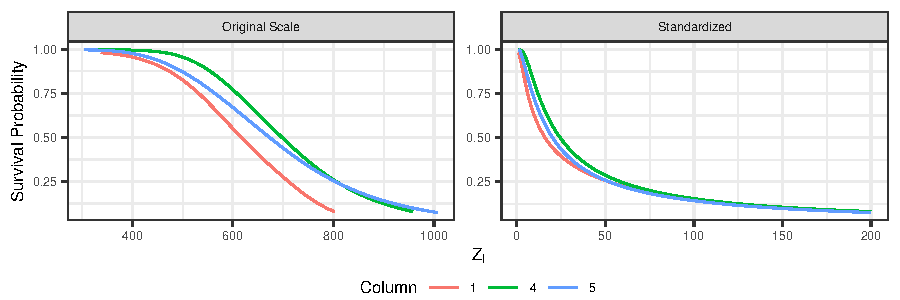
\includegraphics[height=0.8\frametextheight,width=0.9\textwidth]{./ch1/images/condsurv_1d}
  \end{center}
\end{frame} % Conditional Survival 1d

\begin{frame}
    \frametitle{IVT - Conditional Survival 2d (selected)}
    \begin{minipage}{.49\textwidth}
        \centering
        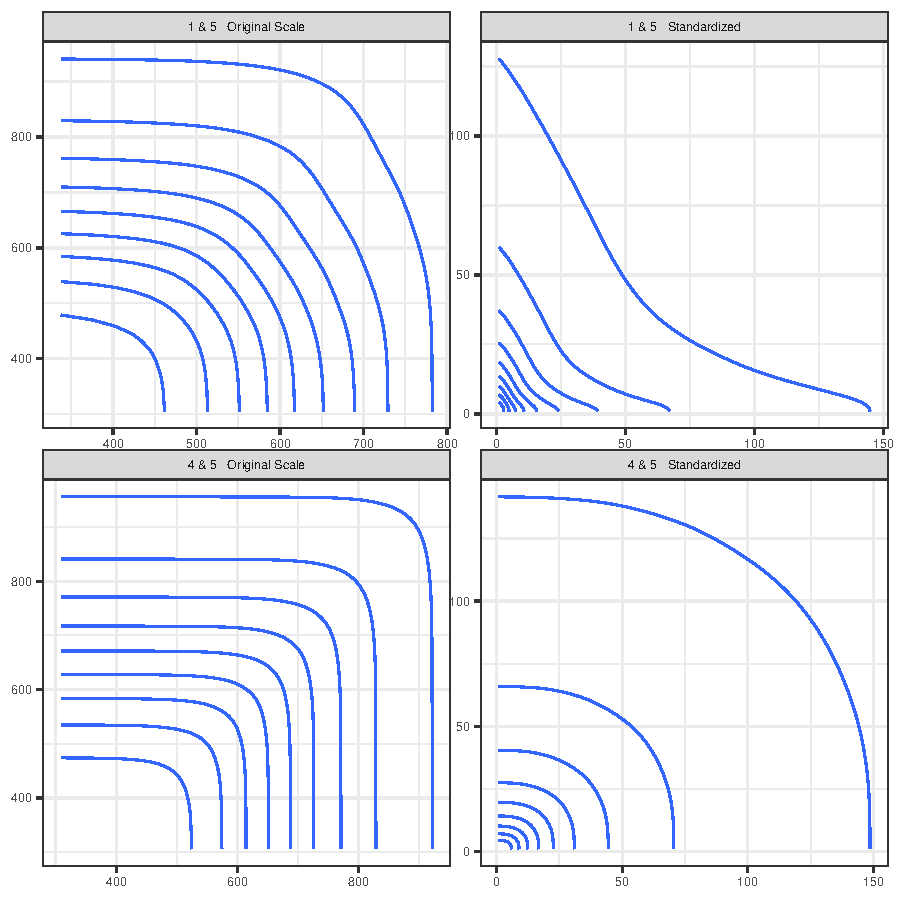
\includegraphics[height=\frametextheight]{./ch1/images/condsurv_2d}
    \end{minipage}
    \begin{minipage}{.49\textwidth}
    Extremal Dependence
        \begin{itemize}
            \item Low between 1 \& 5
            \item High between 4 \& 5
        \end{itemize}
    \end{minipage}
\end{frame} % Conditional Survival 2d


\subsection*{Novelty Detection}

\begin{frame}
  \frametitle{Classical Anomaly Detection Methods}
  \label{ndpg:anomalymethods}
  \begin{itemize}
    \item Clustering methods
      \begin{itemize}
        \item Linkage-based (single, \dots, complete)~\citep{ackerman2010}
        \item Centroid-based ($k$-Means)~\citep{hartigan1979} 
        \item Density-based (DBSCAN)~\citep{ester1996}
      \end{itemize}
    \item Non-statistical Models
      \begin{itemize}
        \item Isolation Forest~\citep{liu2000}
        \item One-class SVM~\citep{chang2011}
        \item Local Outlier Factor~\citep{breunig2000}
      \end{itemize}
    \item Statistical Models
      \begin{itemize}
        \item Density Estimation routines (GMM's, KDE, KNN)
      \end{itemize}
  \end{itemize}
  \hyperlink{ndpg:anomaly}{\beamerbutton{Anomalies}}
\end{frame} % Anomaly Detection Methods

\begin{frame}
    \frametitle{Angular Data Model}
    \label{ndpg:angulardatamodel}
    {\small 
    \begin{itemize}
    \item The Model
    \[
        \begin{aligned}
        \bm{y}_n \mid \bm{\alpha}_n &\sim \mathcal{PG}_p
                \left(\bm{y}\mid\bm{\alpha}_n, \bm{1}\right)\\
        \bm{\alpha_n} &\sim G\\
        G &\sim \mathcal{PY}\left(\omega, \eta, G_0\right)\\
        \end{aligned}
        ~\hspace{1cm}
        \begin{aligned}
        G_0 &= \mathcal{LN}_D\left(\bm{\alpha}\mid\bm{\mu},\Sigma\right)\\
        \mu &\sim \mathcal{N}_D\left(\bm{0},\bm{1}\right)\\
        \Sigma &\sim \mathcal{IW}_D\left(\nu, \Psi\right).
        \end{aligned}
    \]
    \item Stick-breaking Weight - Full Conditional
    \[
    \rho_{\jmath} \mid \bm{n} \sim \text{Beta}\left(1 + C_{\jmath} - \omega, 
            \eta + \sum_{k > \jmath} C_k + \jmath \omega\right)
    \]
    %\pause
    \item Cluster weights
    \[
        \pi_{\jmath} := \rho_{\jmath} \prod_{k < \jmath}(1 - \rho_k)
    \]
    %\pause
    \item Cluster Identity - Full Conditional
    \[
    \mathbb{P}\left[\gamma_n = \jmath \mid \bm{\pi},\bm{\alpha}\right] =
            \frac{\pi_{\jmath}\;\mathcal{PG}_p\left(\bm{y}_n\mid\bm{\alpha}_{\jmath},\bm{1}\right)}{
                \sum_{k = 1}^J \pi_k\;
                \mathcal{PG}_p\left(\bm{y}_n\mid\bm{\alpha}_k,\bm{1}\right)}
    \]
    \end{itemize}
    }
    \hyperlink{ndpg:estimationofangularscore}{\beamerbutton{Estimation of Angular Score}}
\end{frame} % Angular Distribution

\begin{frame}
    \frametitle{Novelty Scores - Calculation}
    \label{ndpg:noveltyscoresdetail}
    {\footnotesize
    \begin{enumerate}
        \item[h$k$nn]
        \[
        \mathcal{S}_{n,\bm{\nu}}^{\text{h$k$nn}} = 
            \frac{N\,\pi^{\frac{D-1}{2}}}{k\,\Gamma\left(\frac{D-1}{2} + 1\right)}
            \;R_{k}\left(\tilde{\mathbb{E}}[\bm{\nu}_n]\right)^{D-1}
        \]
        %\pause 
        \item[hkde]
        \[
        \mathcal{S}_{n,\bm{\nu}}^{\text{hkde}} = \mathbb{E}_{\bm{\nu}^*}\left[
            \exp\left\lbrace
            -\frac{1}{2}\left(
            \frac{g(\tilde{\mathbb{E}}[\bm{\nu}_n], \bm{\nu}^*)}{\hat{h}}
            \right)^2
            \right\rbrace
            \right]^{-1} \approx \left[\frac{1}{K}\sum_{k = 1}^{K}
                \exp\left\lbrace-\frac{1}{2}\left(
                \frac{g(\tilde{\mathbb{E}}[\bm{\nu}_n],\bm{\nu}_k^*)}{\hat{h}}
                \right)^2\right\rbrace\right]^{-1}
        \]
        %\pause
        \item[lhkde]
        \[
        \mathcal{S}_{n,\bm{\nu}}^{\text{lhkde}} = 
            \mathbb{E}_{\bm{\nu}^*,\bm{\nu}_n}\left[
            \exp\left\lbrace
            -\frac{1}{2}\left(
            \frac{g(\bm{\nu}_n, \bm{\nu}^*)}{\hat{h}}
            \right)^2
            \right\rbrace
            \right]^{-1} \approx \left[
                \frac{1}{K_{\bm{\nu}_n}K_{\bm{\nu}^*}}
                \sum_{\jmath = 1}^{K_{\bm{\nu}_n}}\sum_{k = 1}^{K_{\bm{\nu}^*}}
                \exp\left\lbrace-\frac{1}{2}
                \left(\frac{g(\bm{\nu}_{n,\jmath},\bm{\nu}_{k}^*)}{\hat{h}}\right)^2
                \right\rbrace
                \right]^{-1}
        \]
        %\pause
        \item[lskde]
        \[
        \mathcal{S}_{n,\bm{\pi}}^{\text{lskde}} = \mathbb{E}_{\bm{\pi}_i,\bm{\pi}^*}
        \left[\exp\left\lbrace -\frac{1}{2}\left(
            \frac{\lVert \bm{\pi}_n - \bm{\pi}^*\rVert_1}{\hat{h}}
            \right)^2\right\rbrace
        \right]
        \approx 
        \left[
            \frac{1}{K_{\bm{\pi}^*}K_{\bm{\pi}_n}}\sum_{\jmath=1}^{K_{\bm{\pi}_n}}
                \sum_{k=1}^{K_{\bm{\pi}^*}}\exp\left\lbrace
            -\frac{1}{2}
                \left(\frac{\lVert \bm{\pi}_{n\jmath} - \bm{\pi}_k^*\rVert}{\hat{h}}\right)^2
            \right\rbrace
        \right]^{-1}
        \]
    \end{enumerate}
    }
    \hyperlink{ndpg:noveltyscores}{\beamerbutton{Novelty Scores}}
\end{frame} % Categorical Anomaly Scores

\begin{frame}
    \frametitle{Categorical Data Model}
    \label{ndpg:categoricaldatamodel}
    Let $\bm{c}_m$ be categorical RV with $D_m$ categories in one-hot encoding.  
    then $\mathcal{CDC}(\bm{c}\mid\bm{\alpha}) = 
        \prod_{m = 1}^M \mathcal{DC}(\bm{c}_m\mid\bm{\alpha}_m)$.  
        Then
    \begin{itemize}
    %\pause
    \item Model:
    \[
    \begin{aligned}
      \bm{c}_n \mid \bm{\alpha}_n &\sim 
        \mathcal{CDC}\left(\bm{c}_n\mid\bm{\alpha}_n\right)\\
      \bm{\alpha_n} &\sim G\\
      G &\sim \mathcal{PY}\left(d, \eta, G_0\right)\\
      \end{aligned}
      ~\hspace{1cm}
      \begin{aligned}
      G_0 &= \mathcal{LN}\left(\bm{\alpha}\mid\bm{\mu},\Sigma\right)\\
      \mu &\sim \mathcal{N}\left(\bm{0},\bm{1}\right)\\
      \Sigma &\sim \mathcal{IW}\left(\nu, \Psi\right).
      \end{aligned}
      \]
    %\pause
    \item $\Psi$ is block-diagonal matrix.  Within each $m$-block:
    \begin{itemize}
        \item diagonals set to $\psi_0$
        \item off-diagonals set to $-\psi_0D_m^{-2}$; Covariance of uniform categorical.
    \end{itemize}
    \end{itemize}
    \hyperlink{ndpg:categoricaldistributions}{\beamerbutton{Categorical Distributions}}
\end{frame} % Categorical Data Model 


\subsection*{At Scale}

\begin{frame}
    \frametitle{Threshold Trade-offs}
    \label{exapg:thresholdtradeoffs}
    \begin{center}
        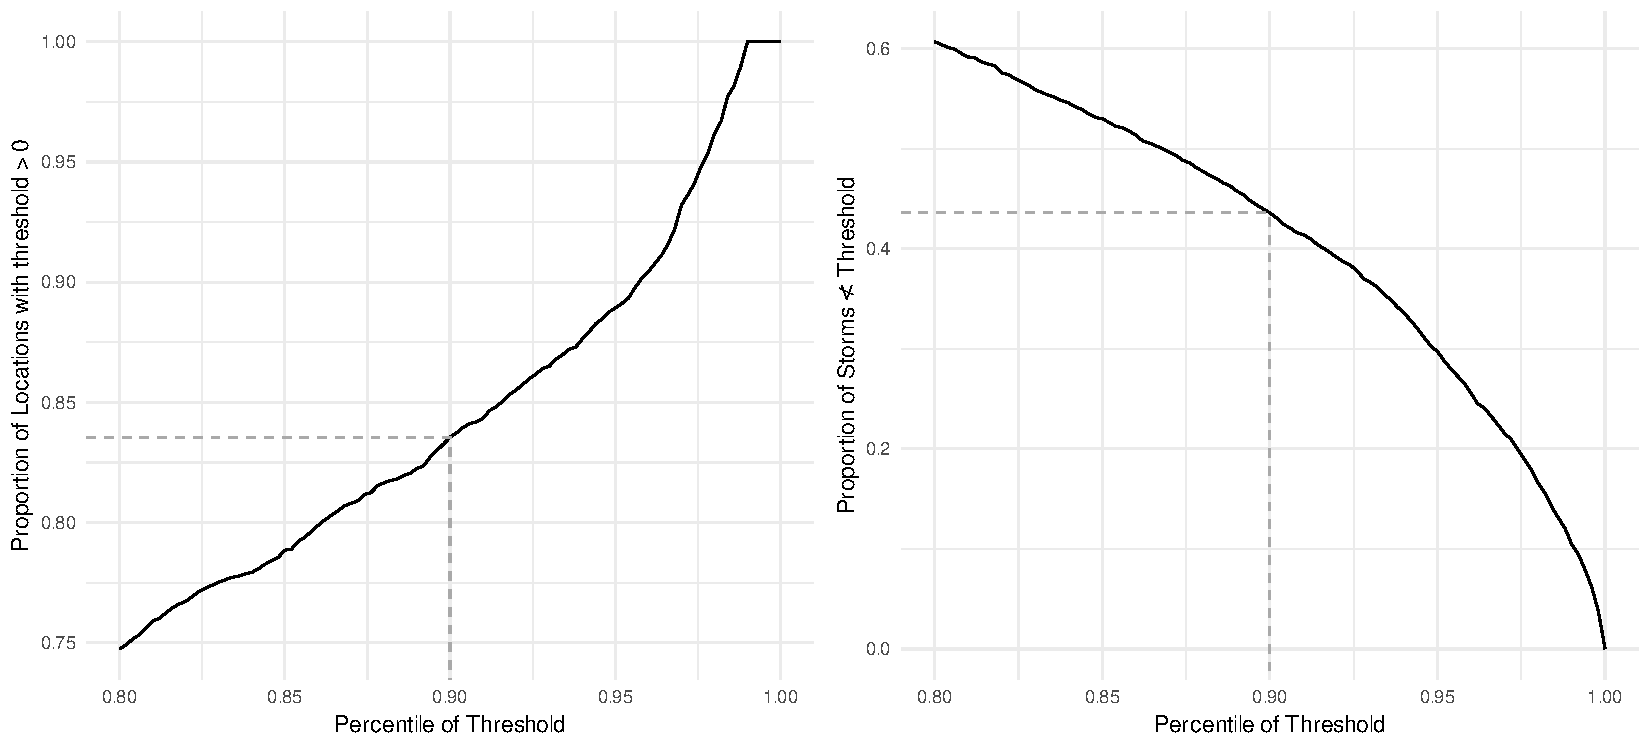
\includegraphics[height = 0.99\frametextheight]{./ch3/plots/explore_threshold}
    \end{center}
\end{frame} % SLOSH Threshold Tradeoffs

\begin{frame}
    \frametitle{A Brief Review}
    \label{exapg:variationalinferencereview}
    \begin{itemize}
    \item The Goal
        \[
            q^*(\bm{\theta}) = \argmin_{q\in\mathcal{Q}}\left\lbrace
            \text{KL}\left(q(\bm{\theta})||f(\bm{\theta}\mid\bm{x})\right) 
            \coloneqq
            \mathbb{E}_{q}\left[\log\left(
            \frac{q(\bm{\theta})}{f(\bm{\theta}\mid\bm{x})}
            \right)\right]
            \right\rbrace.
        \]
    \item Mean Field Variational Bayes
        \[
            q_{\bm{\theta}} = \prod_{\ell \in L}
                q_{\theta_{\ell}}(\theta_{\ell}\mid\psi_{\ell})
        \]
    \item Evidence Lower Bound (ELBO)
        \[
            \mathcal{L}(\bm{\theta}) = 
                \mathbb{E}_q\left[\log f(\bm{x},\bm{\theta}) - 
                \log q(\bm{\theta})\right] 
            = \mathbb{E}_q[\log f(\bm{x},\bm{\theta})] - H,
        \]
    where $H$ is entropy of $q$.
    \end{itemize}
\end{frame} % Brief Review of VI

\begin{frame}
    \frametitle{Optimization Strategy}
    \begin{itemize}
    \item For given family $Q$, optimal $q^*$ means optimal parameter set 
        $\bm{\psi}^*$ such that
        \[
            q^*(\bm{\theta}) = q(\bm{\theta}\mid\bm{\psi}^*)
        \]
    \item Compute the gradient
        \[
            \Delta_{\bm{\psi}} = \frac{\partial}{\partial \psi_{\ell}}
                \left\lbrace\mathbb{E}_{q}\left[\log f(\bm{y}\mid\bm{\theta})\right] 
                    - H(\bm{\psi})\right\rbrace
                \;\;\text{ for }\ell = 1,\ldots,L
        \]
    and move towards optimal point $\Delta_{\bm{\psi}} = \bm{0}$.

    The gradient isn't available in closed form in this model.
    \item Reparametrization Gradient \cite{kingma2022}:
        \begin{enumerate}
            \item Take Samples of $\bm{\theta} = T(\bm{\psi}, \bm{\varepsilon})$ 
                where $\varepsilon \stackrel{iid}{\sim} \mathcal{N}(0,1)$
            \item Move differentiation w.r.t. $\bm{\psi}$ within expectation
            \item Take expectation numerically.
        \end{enumerate}
    \end{itemize}
\end{frame} % Optimization Strategy



\begin{frame}
    \frametitle{VB Initialization}
    {\footnotesize
    \begin{itemize}
        \item Using the Adam Optimizer \cite{kingma2017}
        %\pause
        \item Still dependent on starting position
        %\pause
        \item Starting position strategies
        %\pause
        \begin{enumerate}
            \item[Random] - Random init of cluster parameters and weights
            %\pause
            \item[Uniform] - Random init of cluster parameters, weights initialized such that
            \[
                \mathbb{E}[\bm{\rho}] = \left(\frac{1}{J},\frac{1}{J-1},\ldots,\frac{1}{3},\frac{1}{2}\right)
                \rightarrow \mathbb{E}[\pi_j] = \left(\frac{1}{J},\ldots,\frac{1}{J}\right)
            \]
            %\pause
            \item[Pregamed] - Abridged MCMC init of parameters
            \begin{enumerate}
                \item Random init cluster parameters, weights
                \item Iterative (1) cluster ID's, weights, via Gibbs step
                \item Iterative (2) Resample cluster parameters from initializing distribution
                \item Set parameters:
                \[
                \begin{aligned}
        q_{\alpha_{\jmath d}} &= 
            \mathcal{LN}\left(\psi_{\alpha_{\jmath d \mu}} 
                \coloneqq\log(\alpha_{\jmath d}) - 0.005,\; 
                \psi_{\alpha_{\jmath d}\sigma} \coloneqq0.1\right)\\
        q_{\rho_{\jmath}} &= \text{Logit}\mathcal{N}\left(
        \psi_{\rho_{\jmath}\mu} \coloneqq\psi(\zeta_{\rho_{\jmath} 1}) - \psi(\zeta_{\rho_{\jmath} 2}), \;
            \psi_{\rho_{\jmath}\sigma^2} \coloneqq\psi^{\prime}(\zeta_{\rho_{\jmath} 1}) +
                \psi^{\prime}(\zeta_{\rho_{\jmath} 2})
            \right)
        \end{aligned}   
                \]
                where $\psi(\cdot)$ and $\psi^{\prime}(\cdot)$ are 
                    digamma and trigamma functions, respectively.
            \end{enumerate}
        \end{enumerate}
    \end{itemize}
    }
\end{frame} % VB Initialization

\begin{frame}
    \frametitle{Model Fidelity for Initialization Strategies}
    \begin{center}
    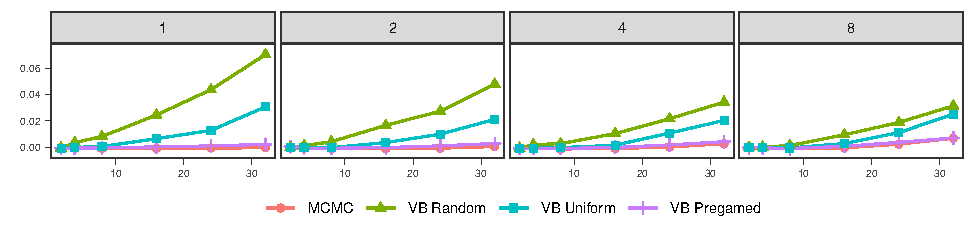
\includegraphics[width = 0.99\textwidth]{./ch3/plots/energy_score}
    \end{center}
\end{frame} % VB Performance


\begin{frame}
    \frametitle{Conditional Survival Curves (Regression, Real)}
    \begin{center}
        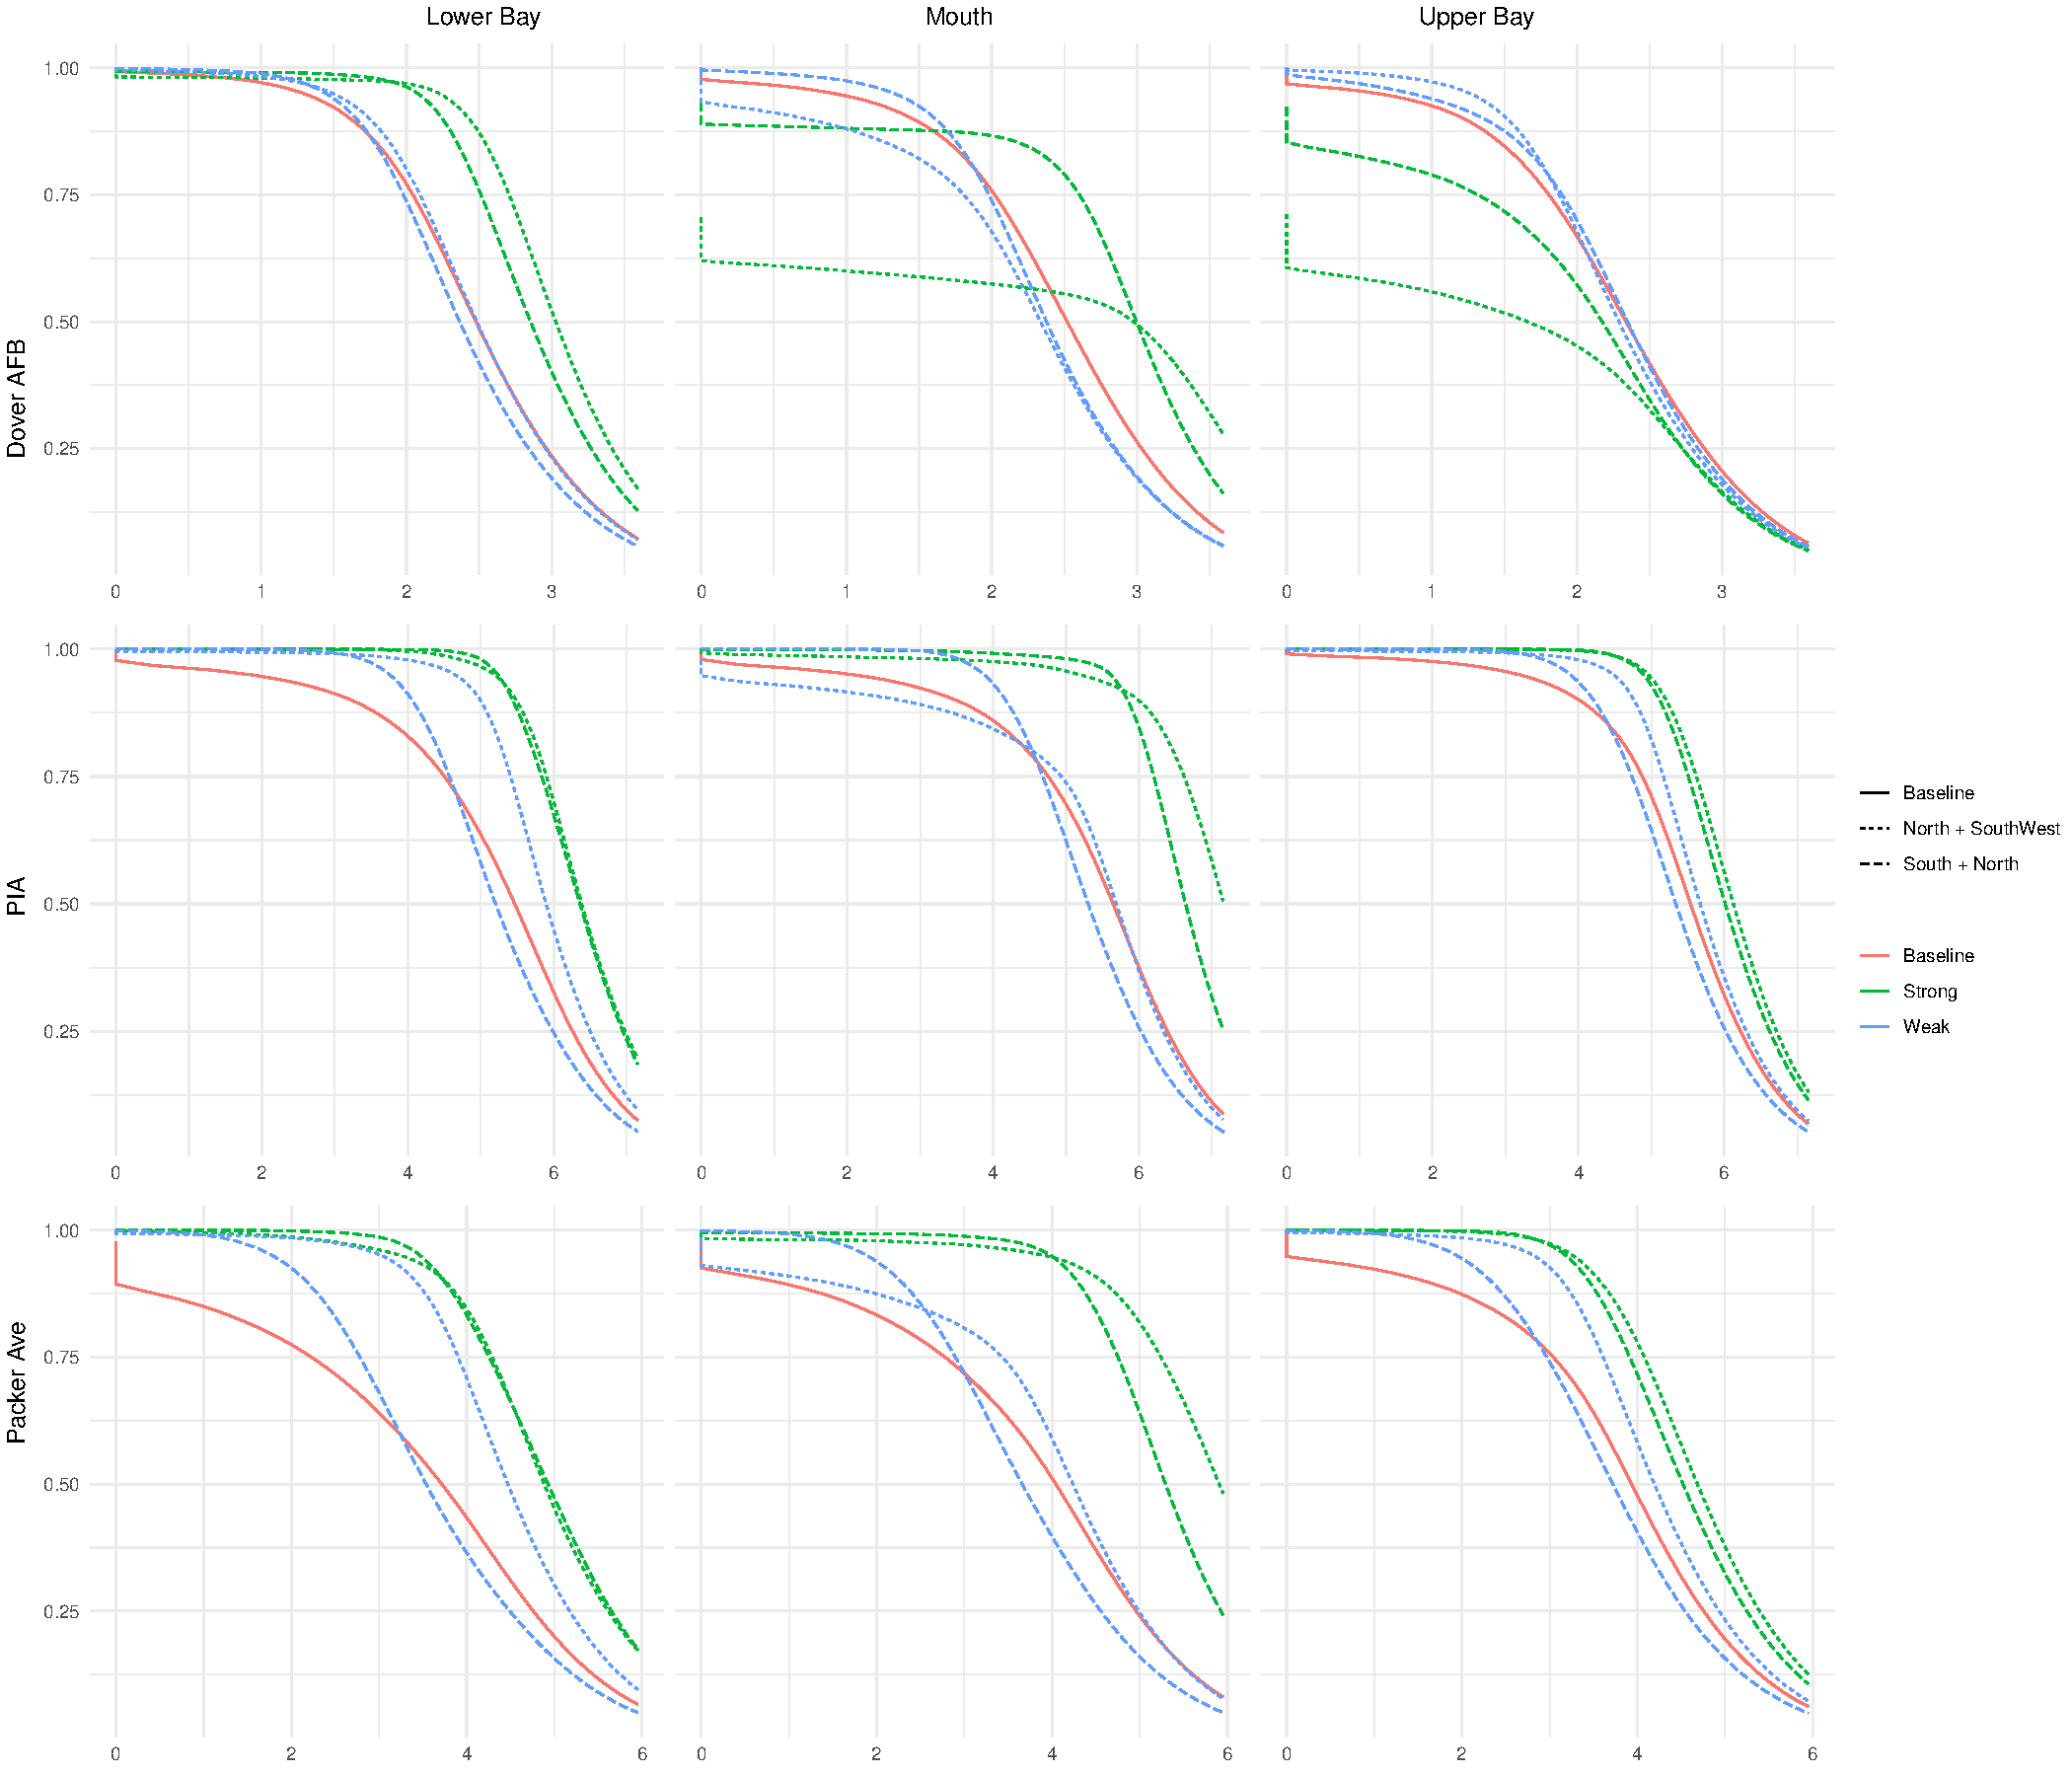
\includegraphics[height=0.99\frametextheight]{./ch3/plots/condsurv_reg/condsurv_reg_1d_real}
    \end{center}
\end{frame}


\begin{frame}
    \frametitle{Conditional Survival Surfaces (Regression, Std)}
    \begin{center}
        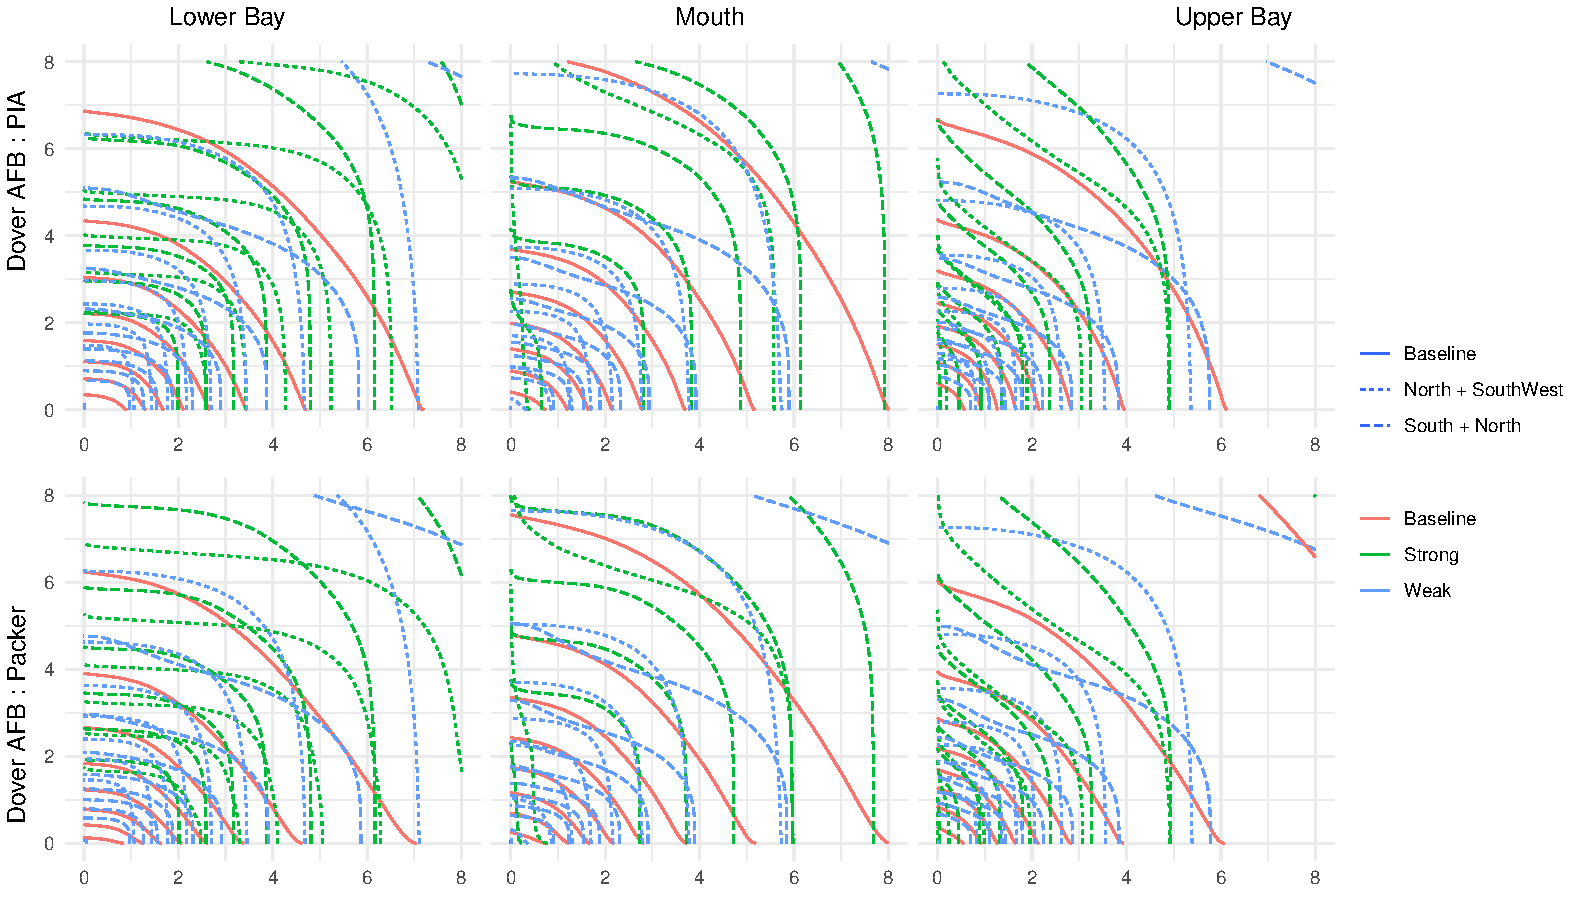
\includegraphics[height=0.99\frametextheight]{./ch3/plots/condsurv_reg/condsurv_reg_2d_std}
    \end{center}
\end{frame}

\begin{frame}
    \frametitle{Conditional Survival Surfaces (Regression, Real)}
    \begin{center}
        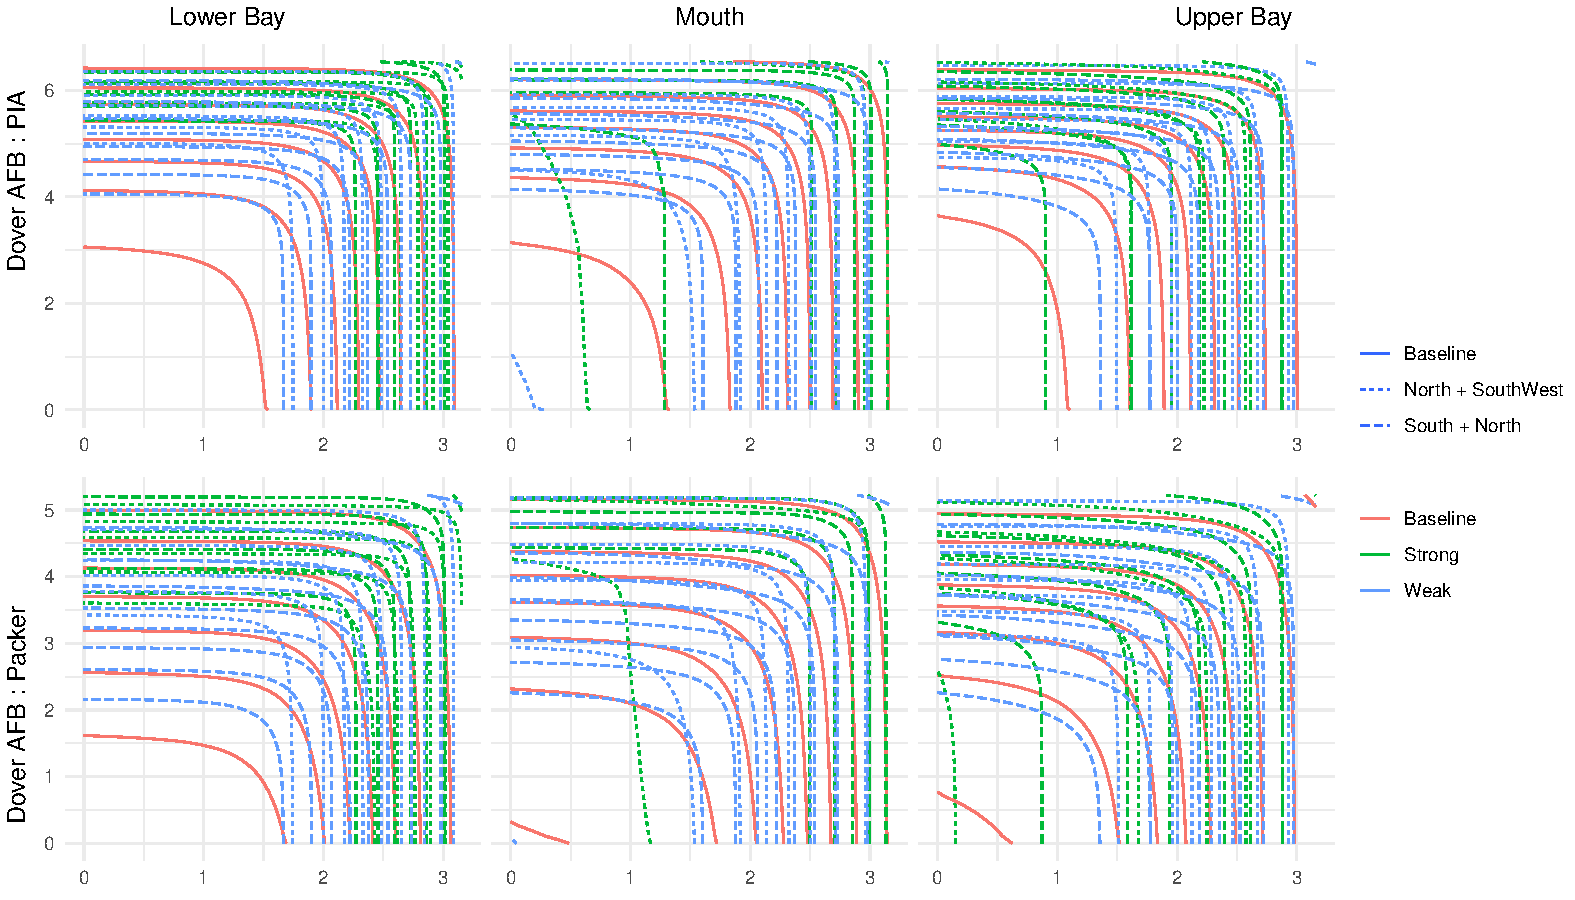
\includegraphics[height=0.99\frametextheight]{./ch3/plots/condsurv_reg/condsurv_reg_2d_real}
    \end{center}
\end{frame}

\end{document}
